\chapter{Model / Experiment Comparison Graphs}
\label{sec:Graphs}

\section{FM Four Room Including Corridor Test Series}

This data set describes a series of tests conducted in a multiple room configuration with more complex gas burner fires than the previous data set.  This study \cite{Heskestad:1986} was included because, in many ways, it is similar to the smoke movement study performed at NBS \cite{Peacock:1988}, and permits comparisons between two different laboratories. In addition, it expands upon that data set by providing larger a time-varying gas burner fires in a room-corridor configuration. Fire size was about up to 1 MW with a total volume of 200 m$^3$. This study was performed to collect data allowing for variations in fire source, ventilation, and geometry in a multi-compartment structure, especially for situations with closed doors.

\begin{figure}[p]
\begin{tabular*}{\textwidth}{l@{\extracolsep{\fill}}r}
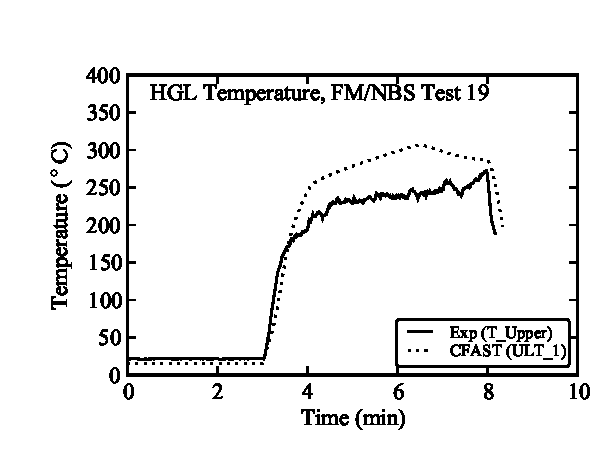
\includegraphics[width=2.6in]{FIGURES/FM_NBS/FM19_1_HGL_Temp} &
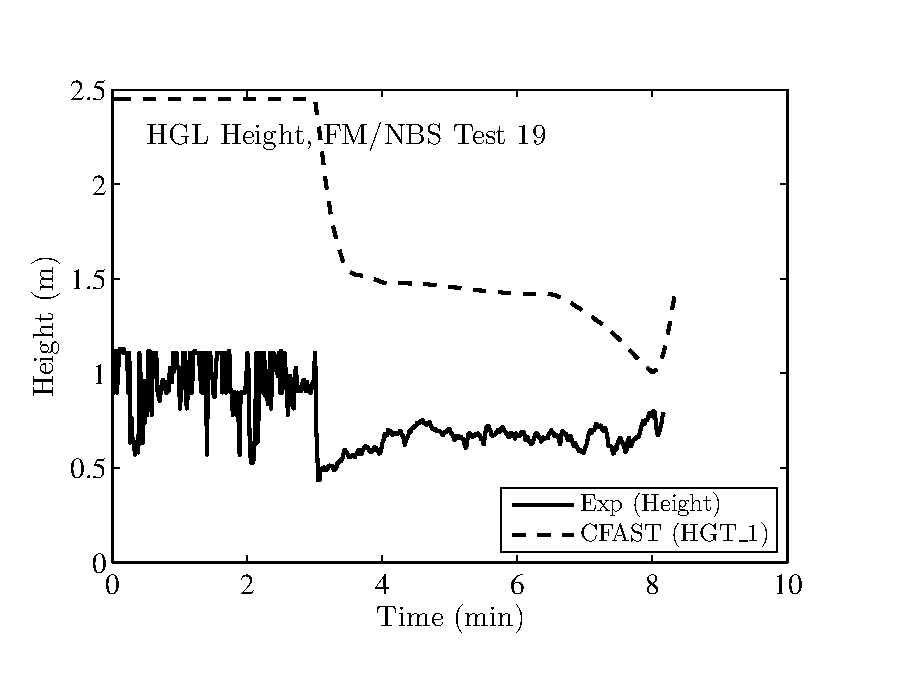
\includegraphics[width=2.6in]{FIGURES/FM_NBS/FM19_1_HGL_Height} \\
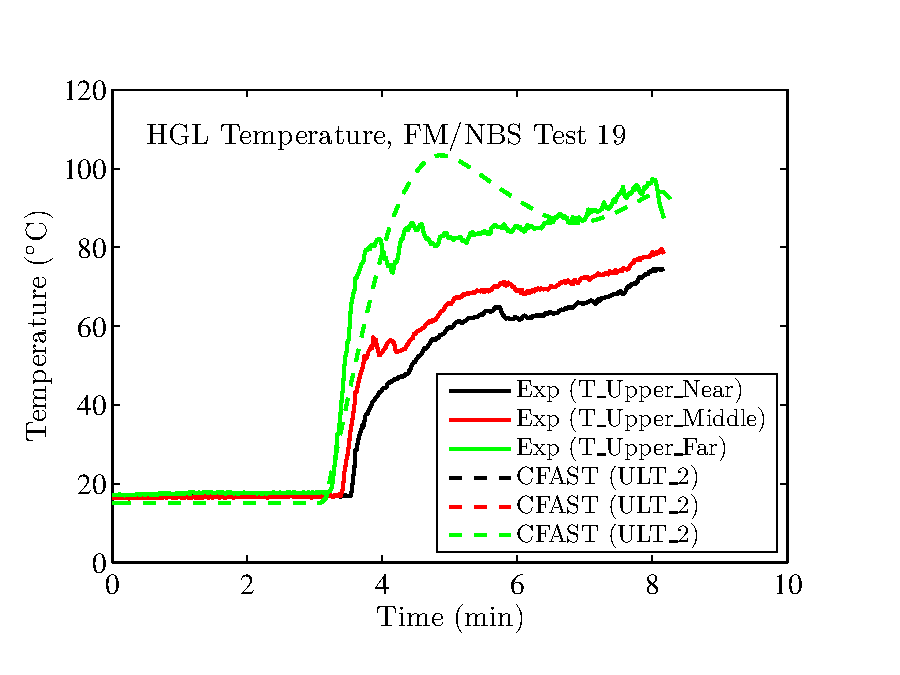
\includegraphics[width=2.6in]{FIGURES/FM_NBS/FM19_2_HGL_Temp} &
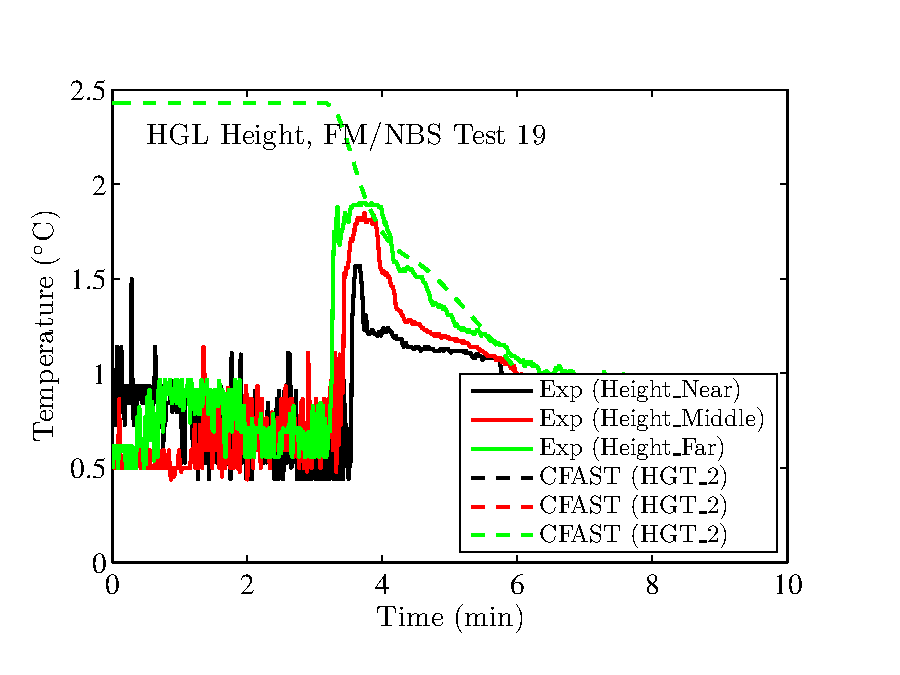
\includegraphics[width=2.6in]{FIGURES/FM_NBS/FM19_2_HGL_Height} \\
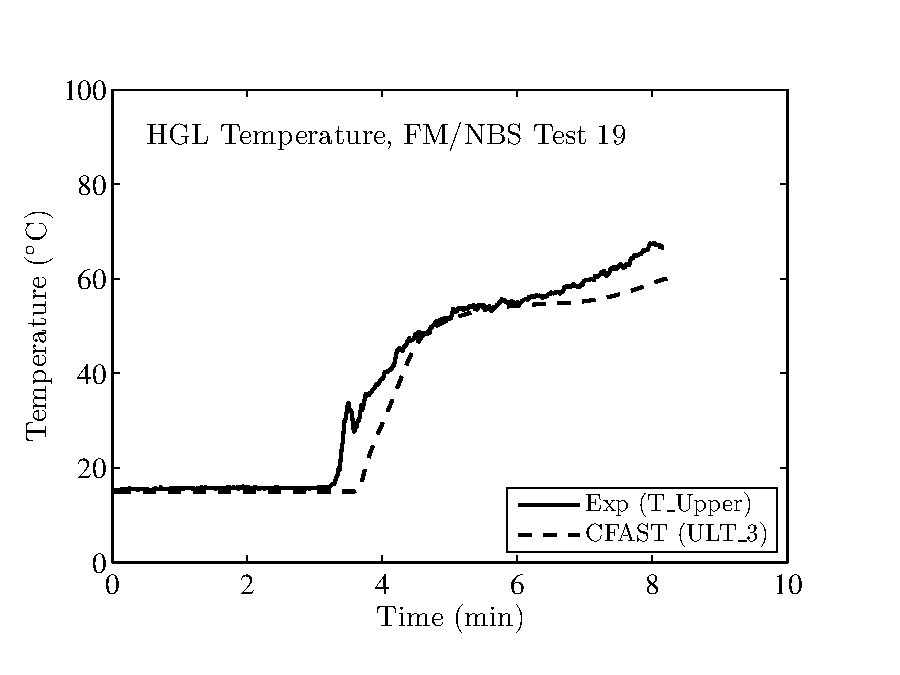
\includegraphics[width=2.6in]{FIGURES/FM_NBS/FM19_3_HGL_Temp} &
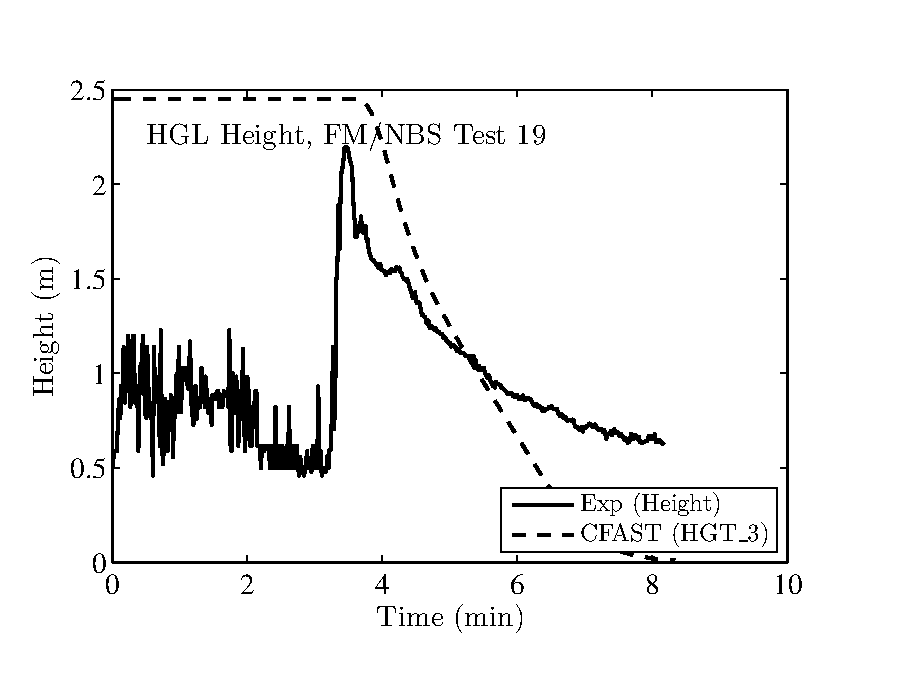
\includegraphics[width=2.6in]{FIGURES/FM_NBS/FM19_3_HGL_Height} \\
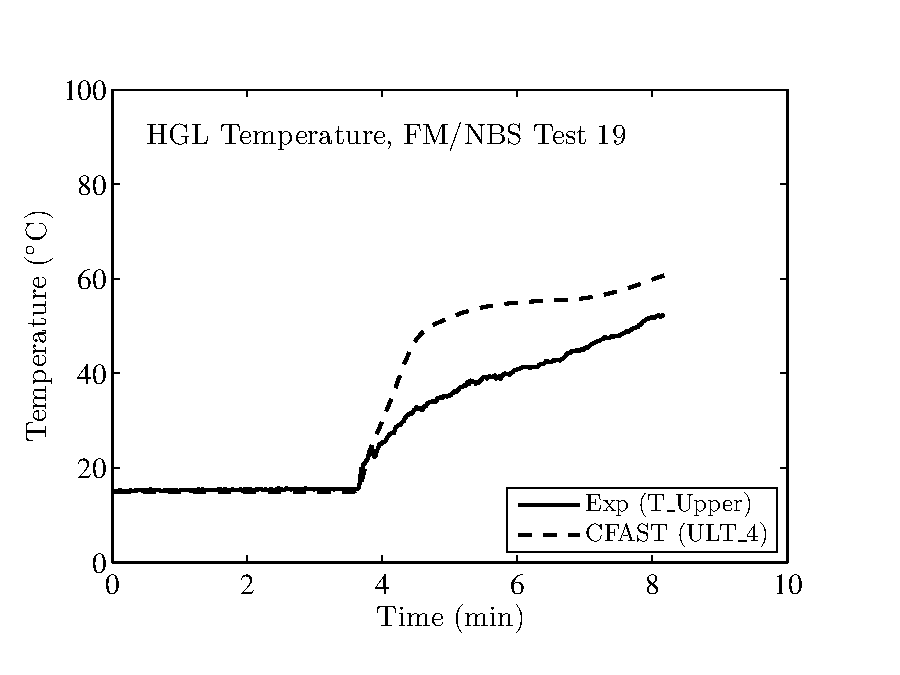
\includegraphics[width=2.6in]{FIGURES/FM_NBS/FM19_4_HGL_Temp} &
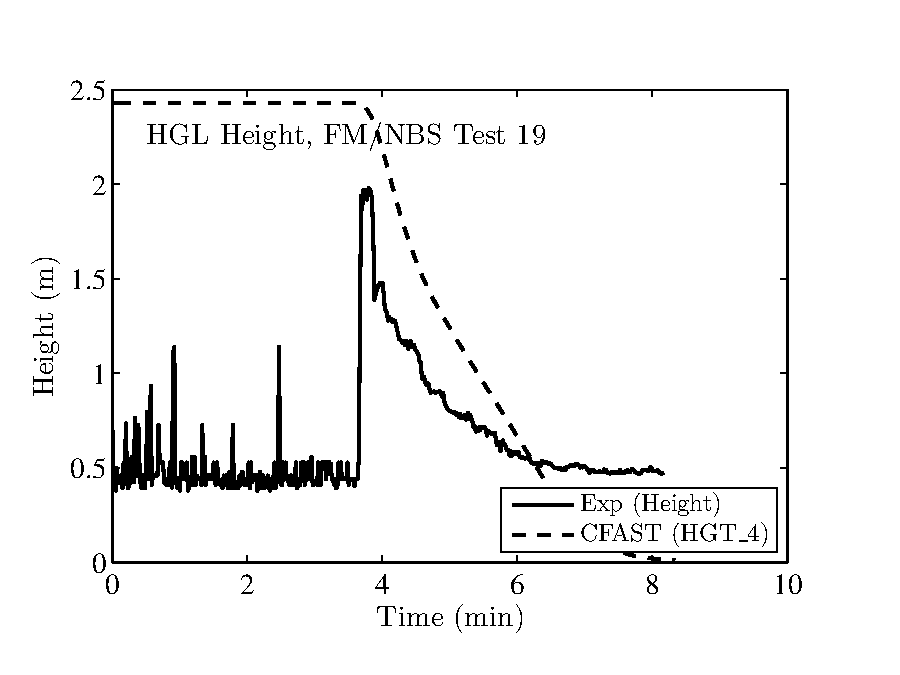
\includegraphics[width=2.6in]{FIGURES/FM_NBS/FM19_4_HGL_Height} \\
\end{tabular*}
\caption{Hot Gas Layer Temperature and Height for the FM/NBS Four Compartment Test 19.} \label{fig:FM_NBS_19_HGL}
\end{figure}

\begin{figure}[p]
\begin{tabular*}{\textwidth}{l@{\extracolsep{\fill}}r}
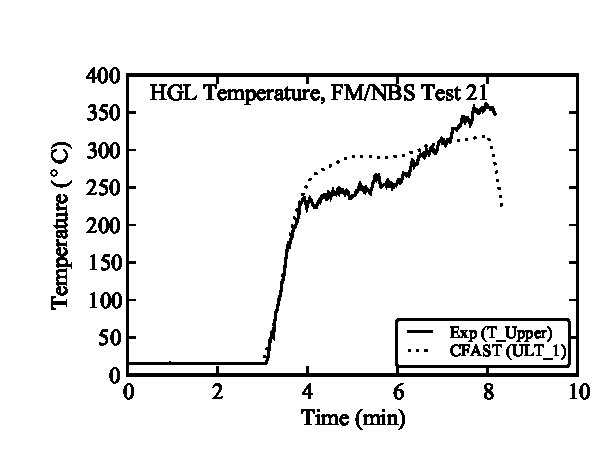
\includegraphics[width=2.6in]{FIGURES/FM_NBS/FM21_1_HGL_Temp} &
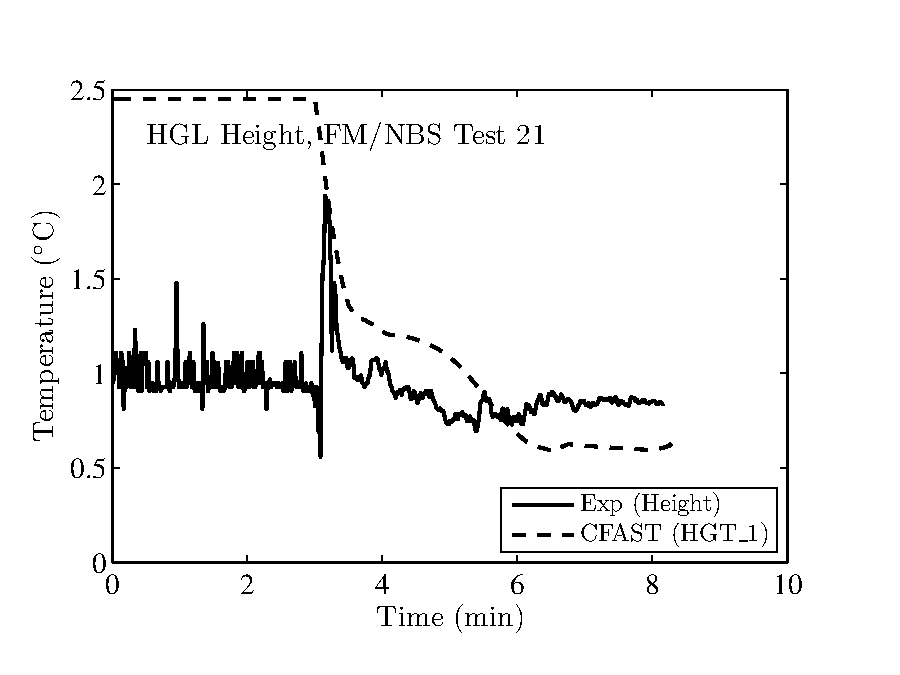
\includegraphics[width=2.6in]{FIGURES/FM_NBS/FM21_1_HGL_Height} \\
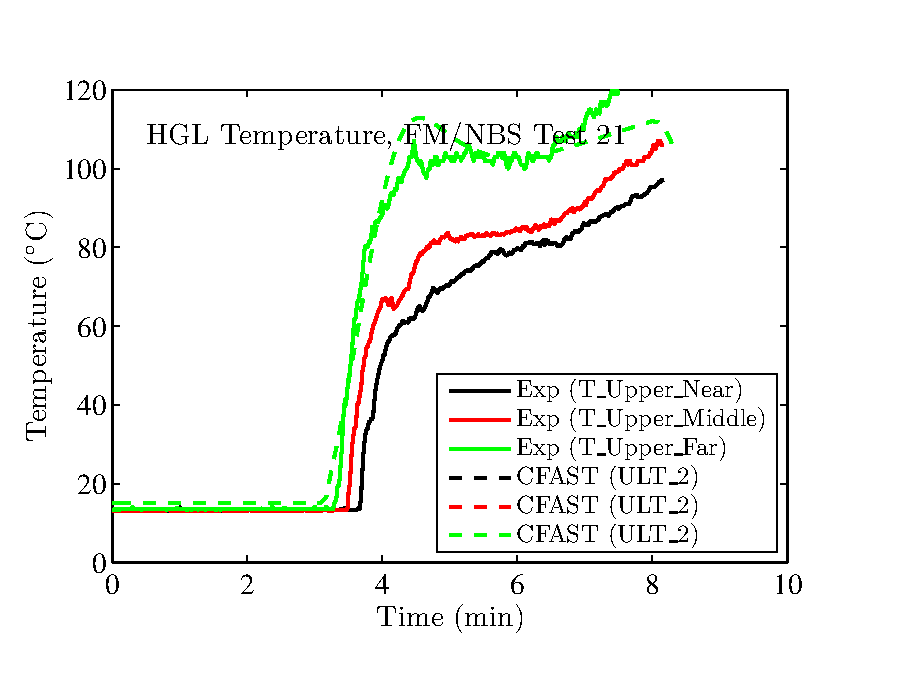
\includegraphics[width=2.6in]{FIGURES/FM_NBS/FM21_2_HGL_Temp} &
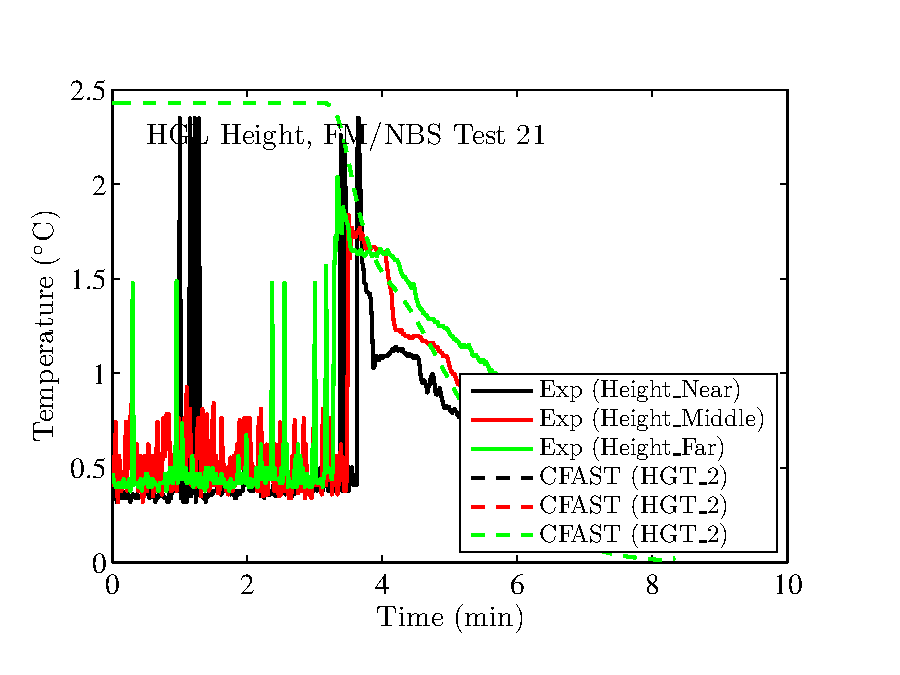
\includegraphics[width=2.6in]{FIGURES/FM_NBS/FM21_2_HGL_Height} \\
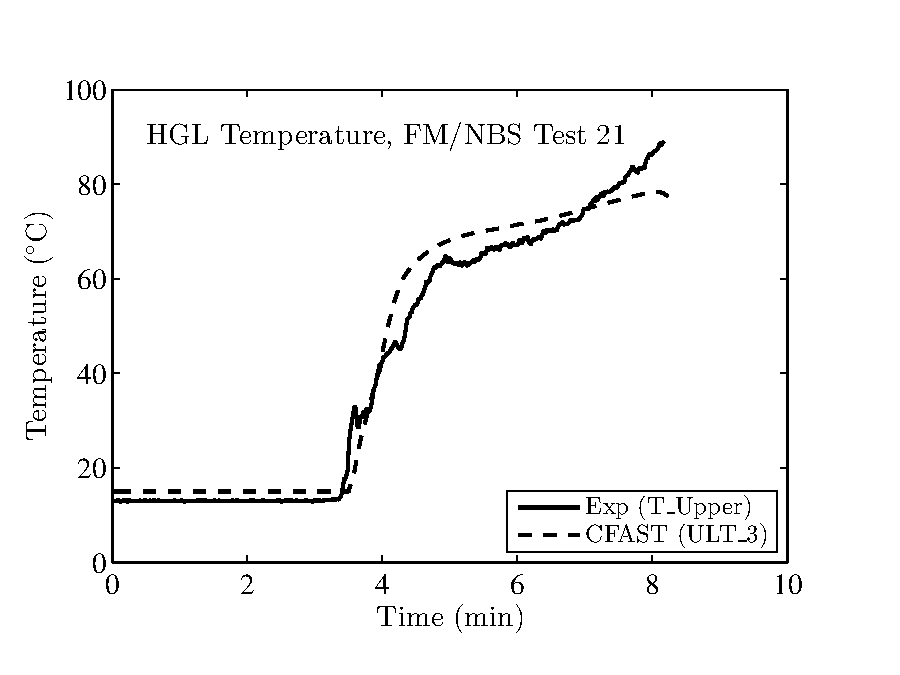
\includegraphics[width=2.6in]{FIGURES/FM_NBS/FM21_3_HGL_Temp} &
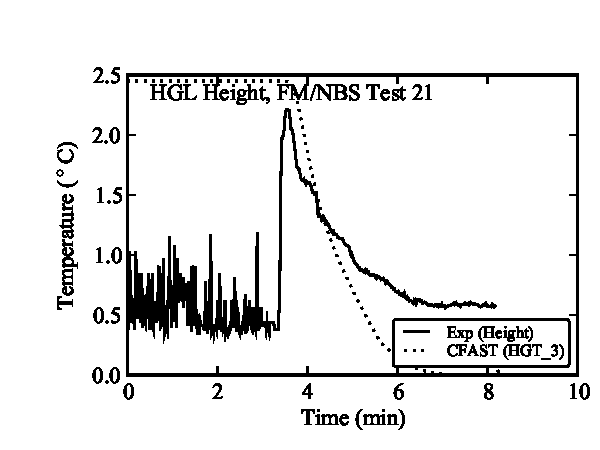
\includegraphics[width=2.6in]{FIGURES/FM_NBS/FM21_3_HGL_Height} \\
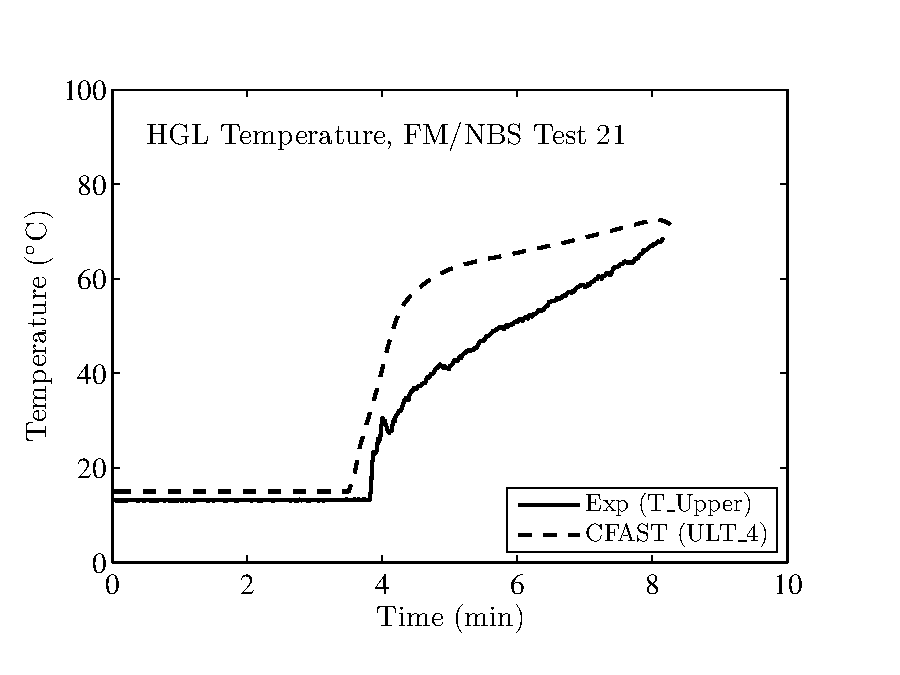
\includegraphics[width=2.6in]{FIGURES/FM_NBS/FM21_4_HGL_Temp} &
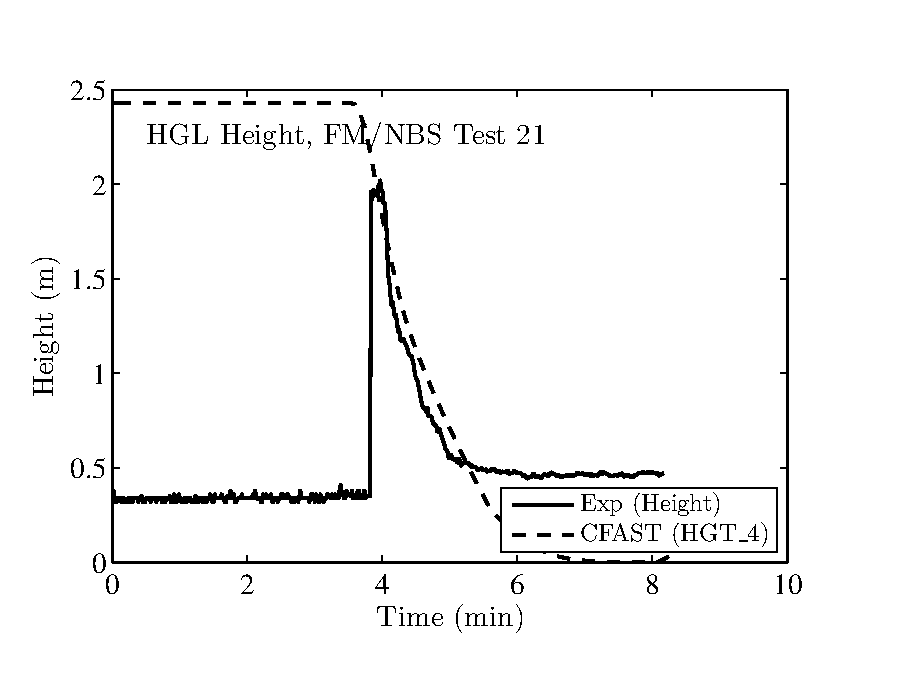
\includegraphics[width=2.6in]{FIGURES/FM_NBS/FM21_4_HGL_Height}
\end{tabular*}
\caption{Hot Gas Layer Temperature and Height for the FM/NBS Four Compartment Test 21.} \label{fig:FM_NBS_21_HGL}
\end{figure}

\begin{figure}[p]
\begin{tabular*}{\textwidth}{l@{\extracolsep{\fill}}r}
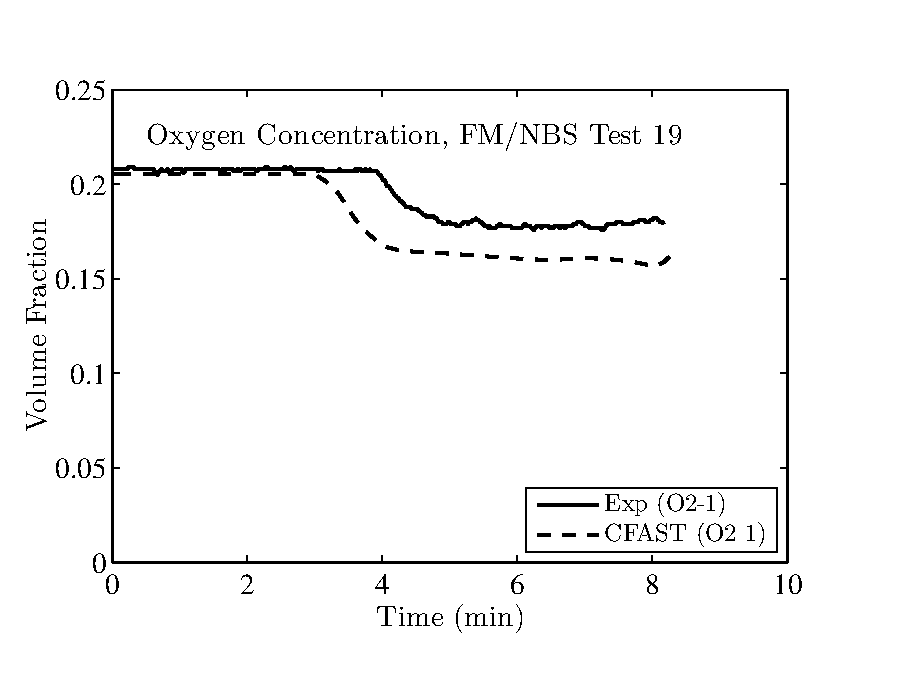
\includegraphics[width=2.6in]{FIGURES/FM_NBS/FM19_1_Oxygen} &
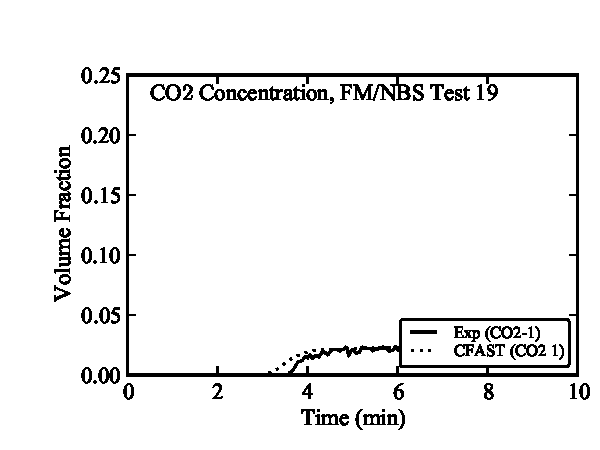
\includegraphics[width=2.6in]{FIGURES/FM_NBS/FM19_1_CO2} \\
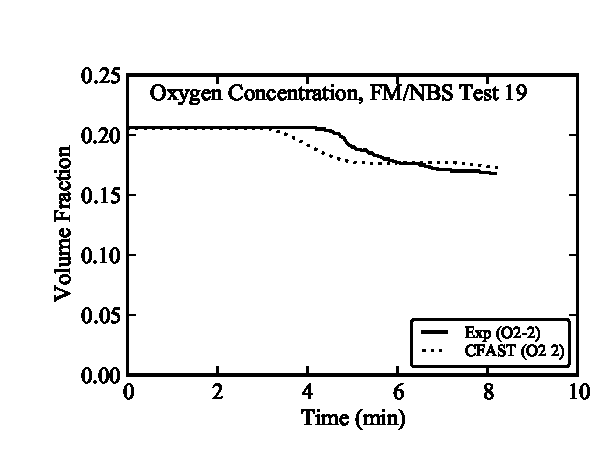
\includegraphics[width=2.6in]{FIGURES/FM_NBS/FM19_2_Oxygen} &
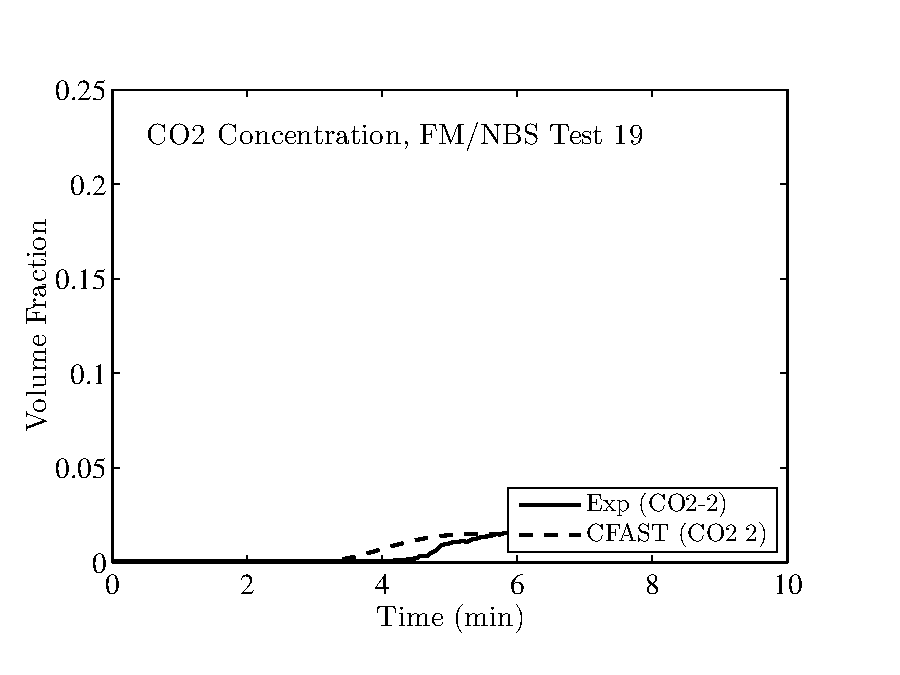
\includegraphics[width=2.6in]{FIGURES/FM_NBS/FM19_2_CO2} \\
 &
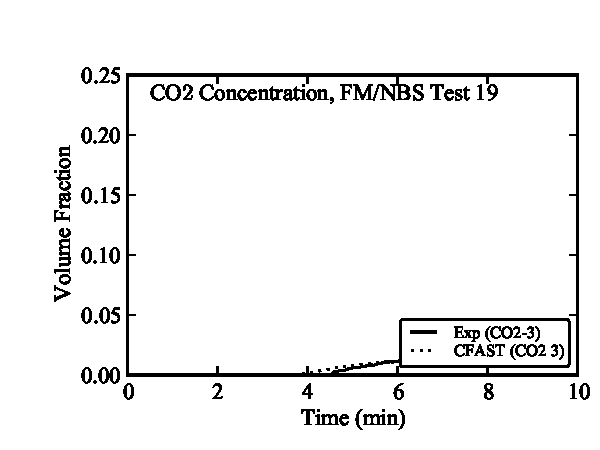
\includegraphics[width=2.6in]{FIGURES/FM_NBS/FM19_3_CO2} \\
&
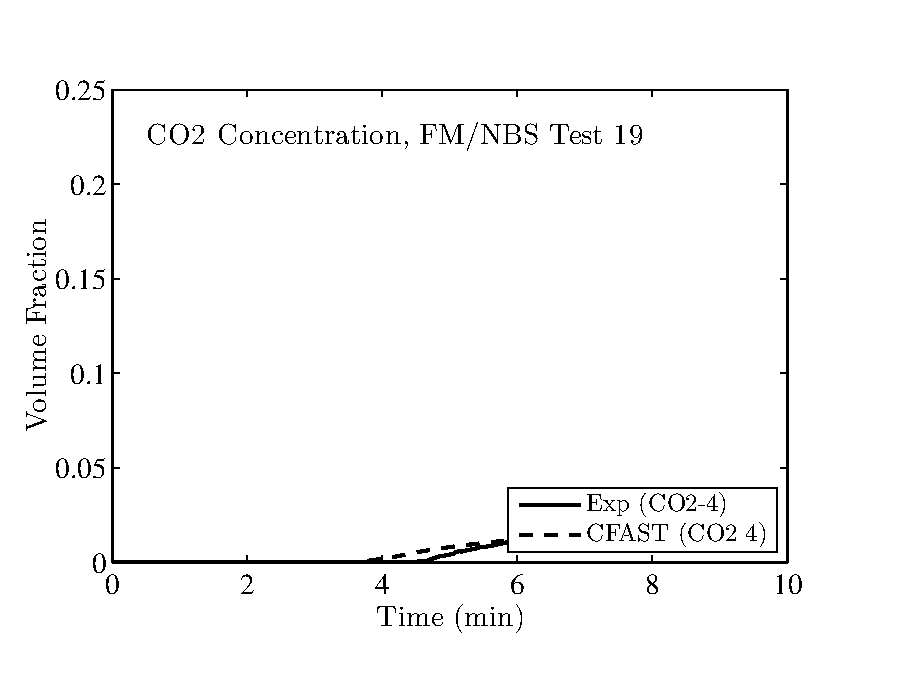
\includegraphics[width=2.6in]{FIGURES/FM_NBS/FM19_4_CO2} 
\end{tabular*}
\caption{Oxygen and Carbon Dioxide Concentration for the FM/NBS Test 19.} \label{fig:FM_SNL_4_Gases}
\end{figure}

\begin{figure}[p]
\begin{tabular*}{\textwidth}{l@{\extracolsep{\fill}}r}
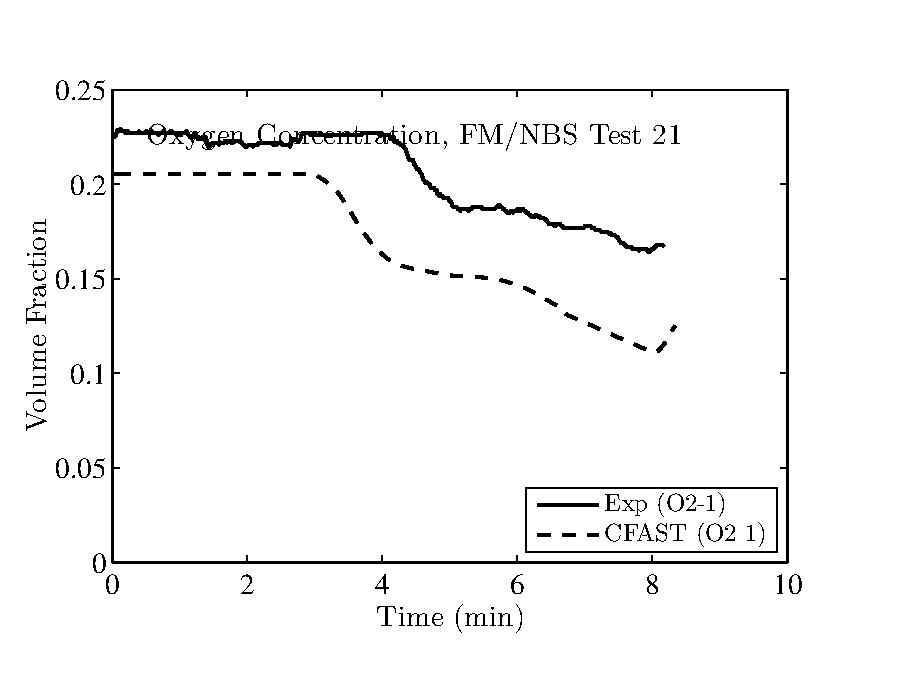
\includegraphics[width=2.6in]{FIGURES/FM_NBS/FM21_1_Oxygen} &
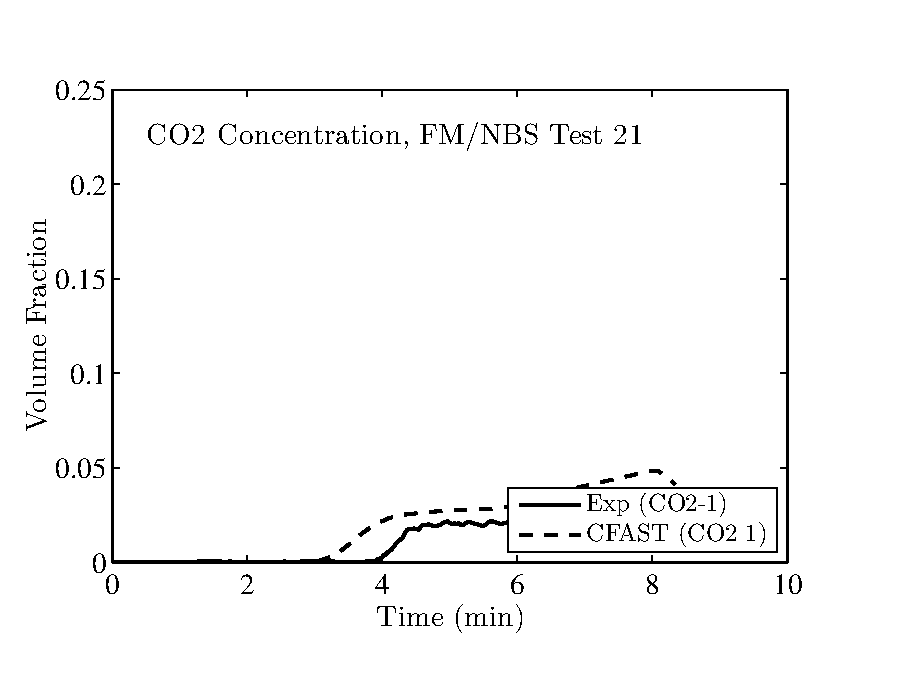
\includegraphics[width=2.6in]{FIGURES/FM_NBS/FM21_1_CO2} \\
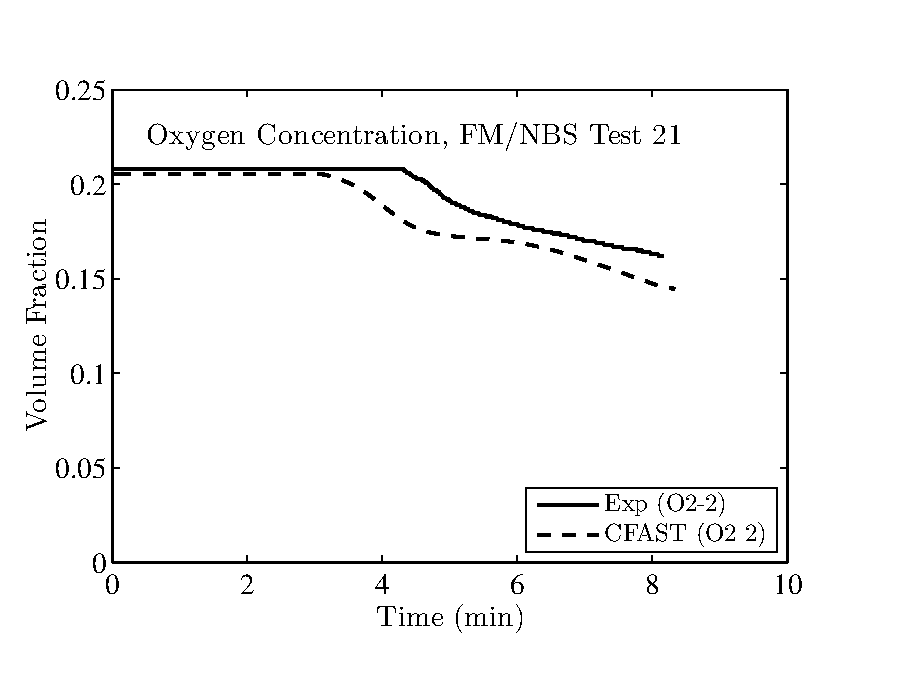
\includegraphics[width=2.6in]{FIGURES/FM_NBS/FM21_2_Oxygen} &
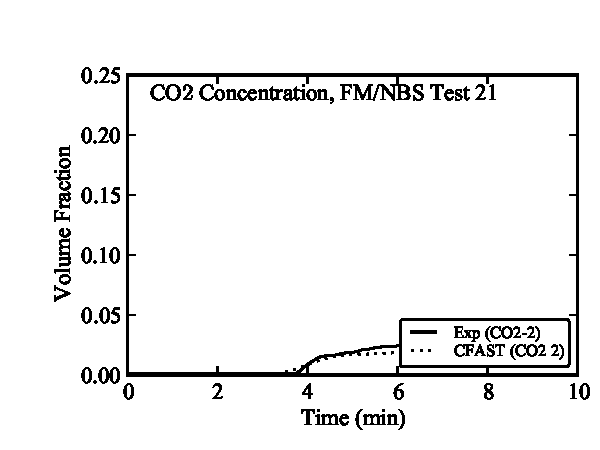
\includegraphics[width=2.6in]{FIGURES/FM_NBS/FM21_2_CO2} \\
 &
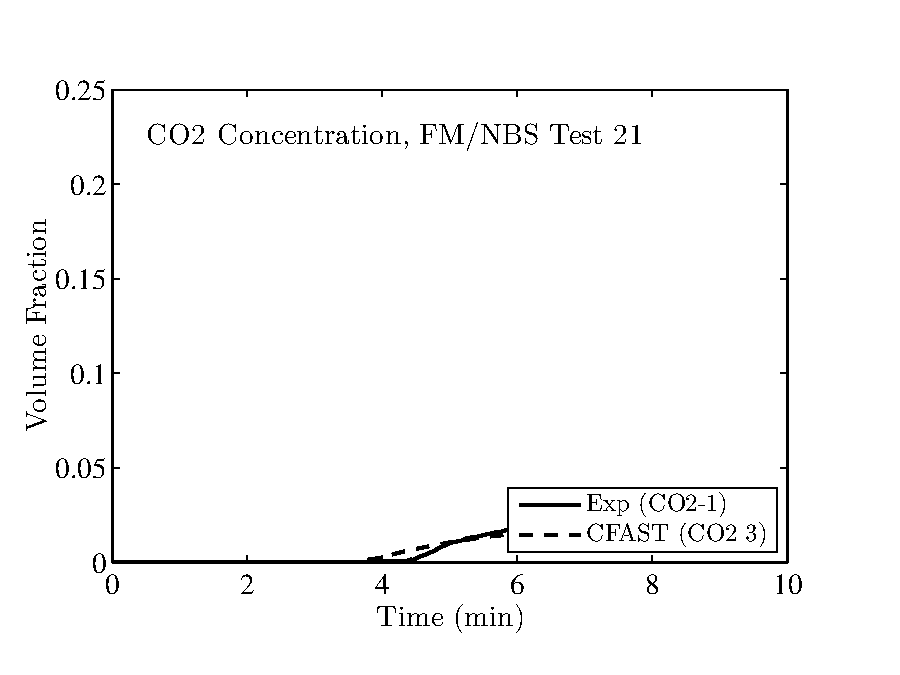
\includegraphics[width=2.6in]{FIGURES/FM_NBS/FM21_3_CO2} \\
&
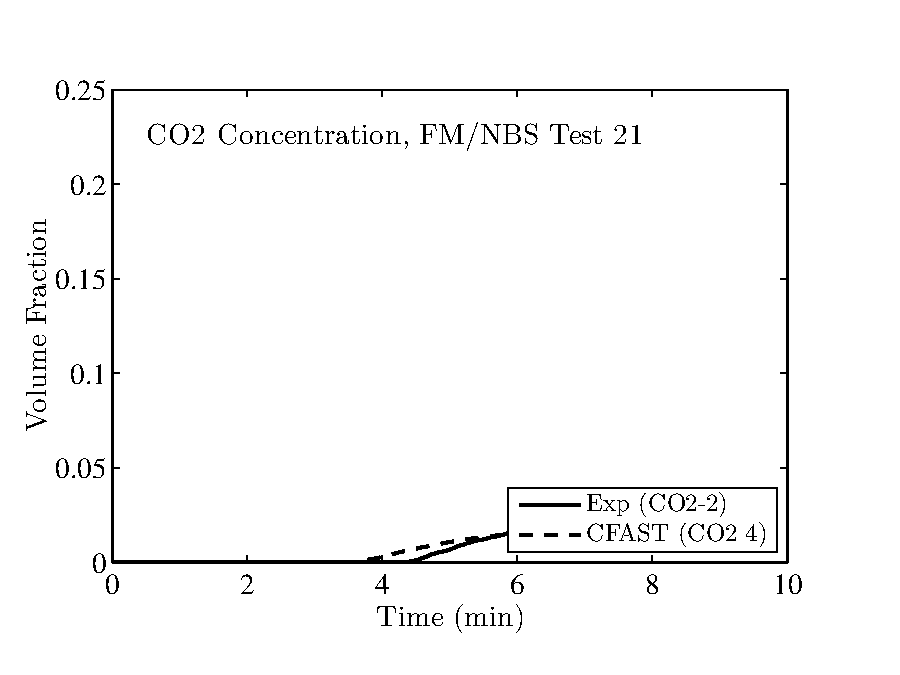
\includegraphics[width=2.6in]{FIGURES/FM_NBS/FM21_4_CO2} 
\end{tabular*}
\caption{Oxygen and Carbon Dioxide Concentration for the FM/NBS Test 21.} \label{fig:FM21_Gases}
\end{figure}

\clearpage

\section{FM/SNL Test Series}

The Factory Mutual and Sandia National Laboratories (FM/SNL) Test Series was a series of 25 fire tests conducted in 1985 for the NRC by Factory Mutual Research Corporation (FMRC), under the direction of Sandia National Laboratories (SNL).  The primary purpose of these tests was to provide data with which to validate computer models for various types of NPP compartments.  The experiments were conducted in an enclosure measuring 18 m x 12 m x 6 m, constructed at the FMRC fire test facility in Rhode Island.  The FM/SNL test series is described in detail, including the types and locations of measurement devices, as well as some results in References \cite{Nowlen:1987, Sandia:1989}.

\begin{figure}[p]
\begin{tabular*}{\textwidth}{l@{\extracolsep{\fill}}r}
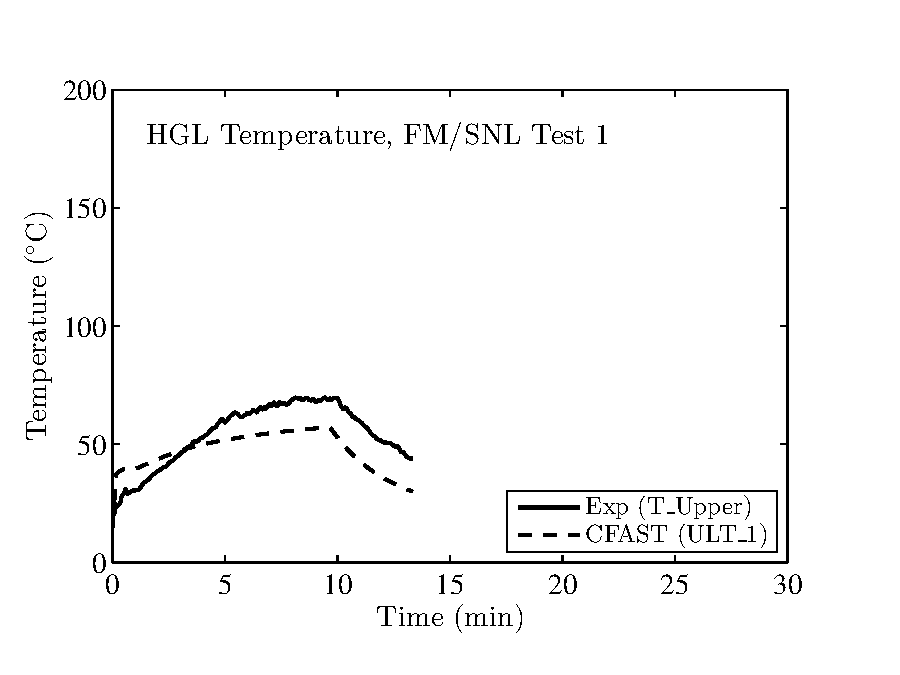
\includegraphics[width=2.6in]{FIGURES/FM_SNL/FM_SNL_01_HGL_Temp} &
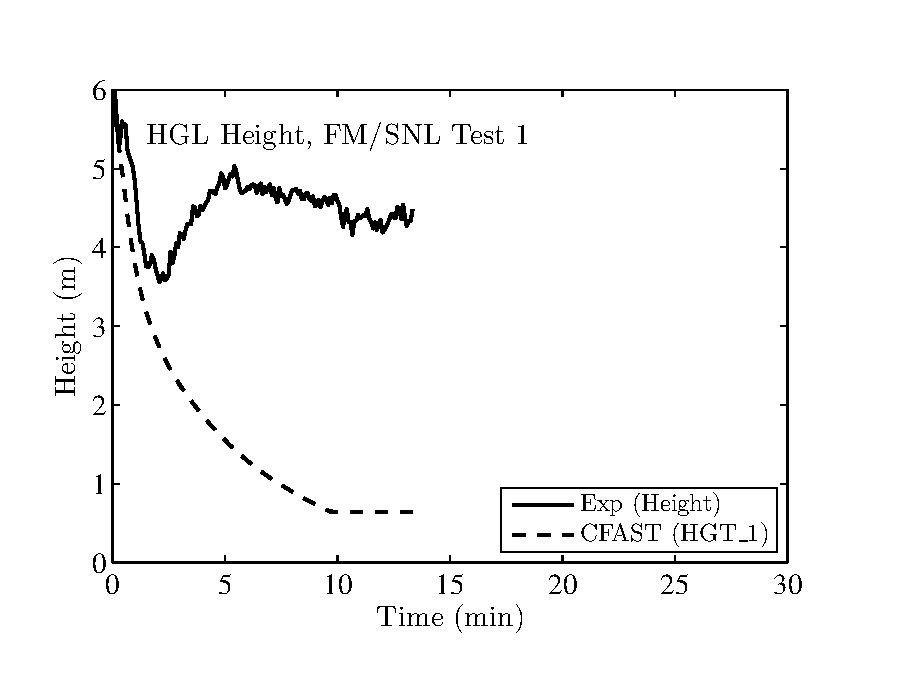
\includegraphics[width=2.6in]{FIGURES/FM_SNL/FM_SNL_01_HGL_Height} \\
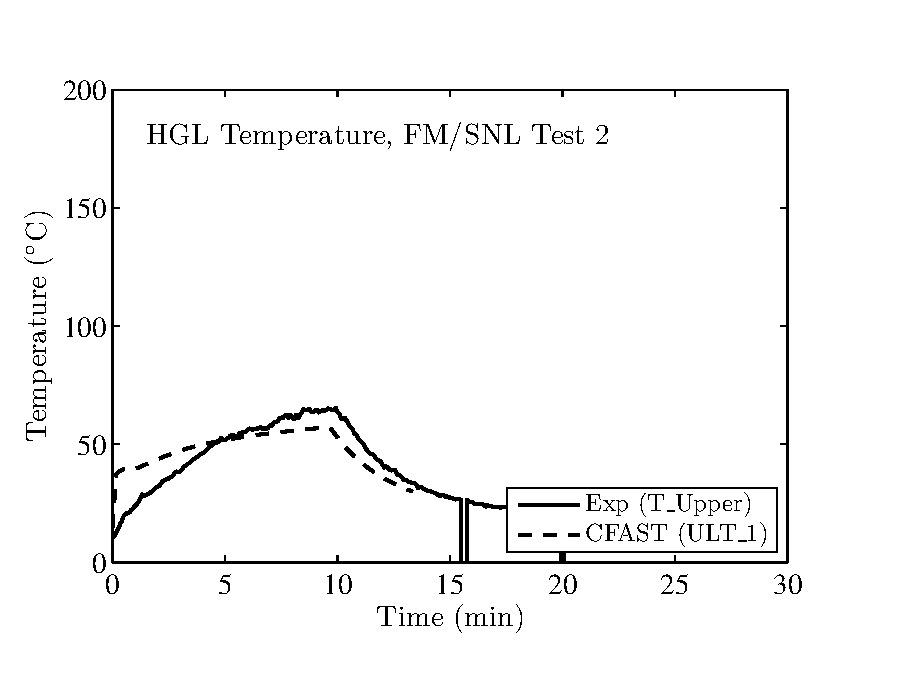
\includegraphics[width=2.6in]{FIGURES/FM_SNL/FM_SNL_02_HGL_Temp} &
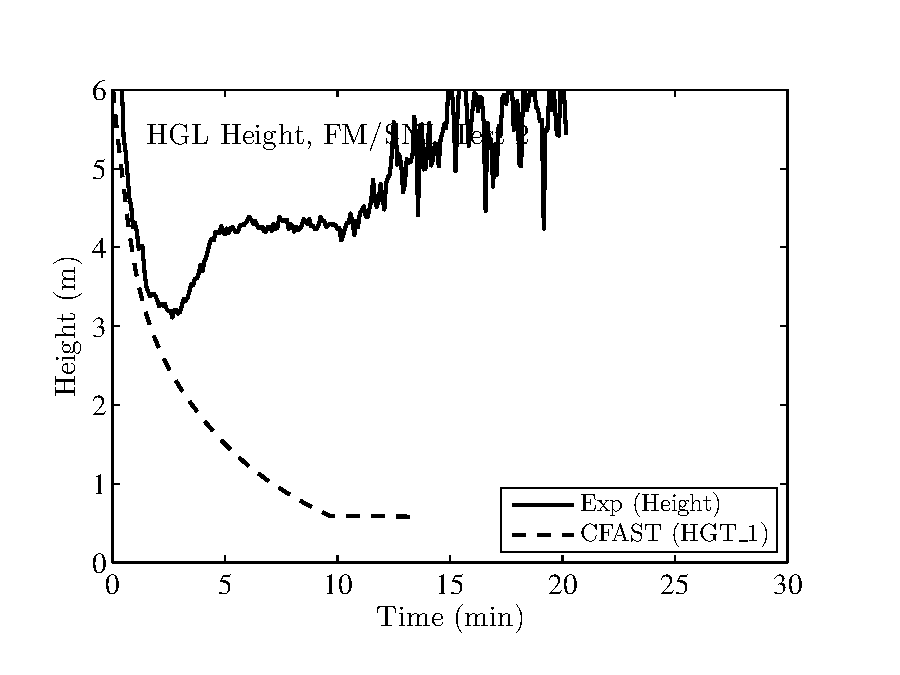
\includegraphics[width=2.6in]{FIGURES/FM_SNL/FM_SNL_02_HGL_Height} \\
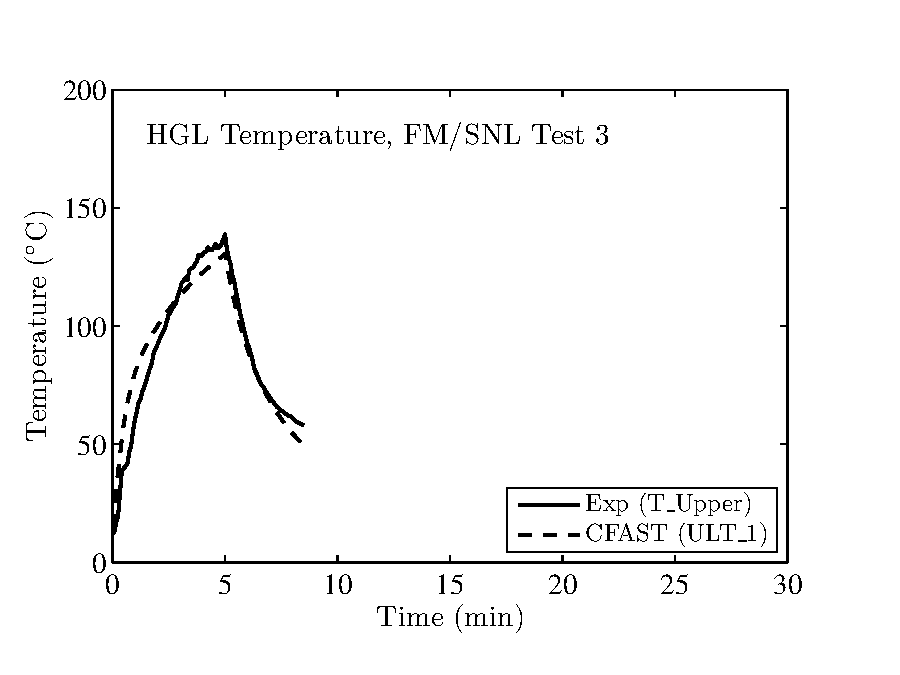
\includegraphics[width=2.6in]{FIGURES/FM_SNL/FM_SNL_03_HGL_Temp} &
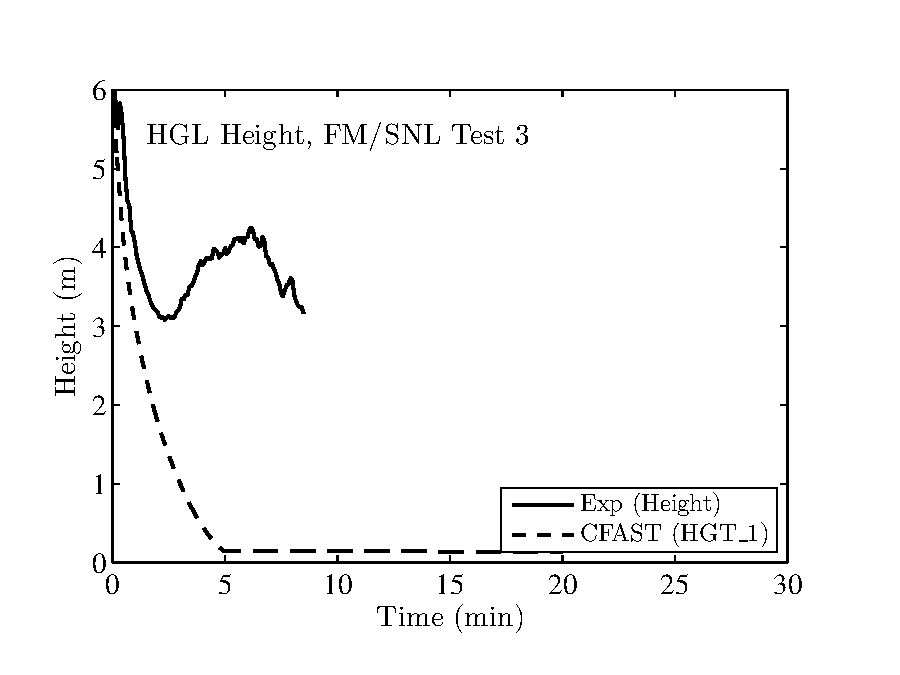
\includegraphics[width=2.6in]{FIGURES/FM_SNL/FM_SNL_03_HGL_Height} \\
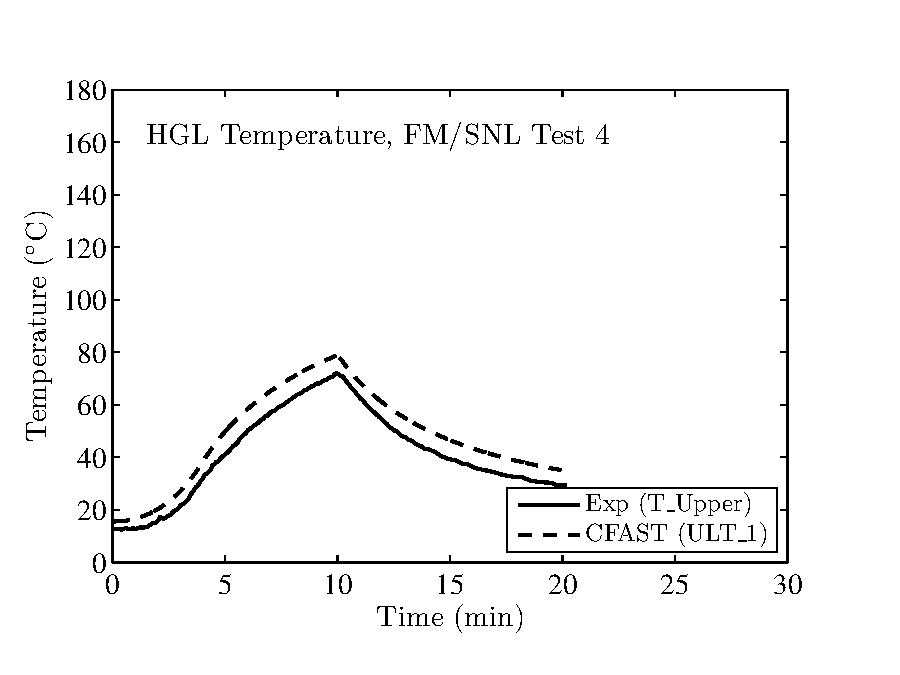
\includegraphics[width=2.6in]{FIGURES/FM_SNL/FM_SNL_04_HGL_Temp} &
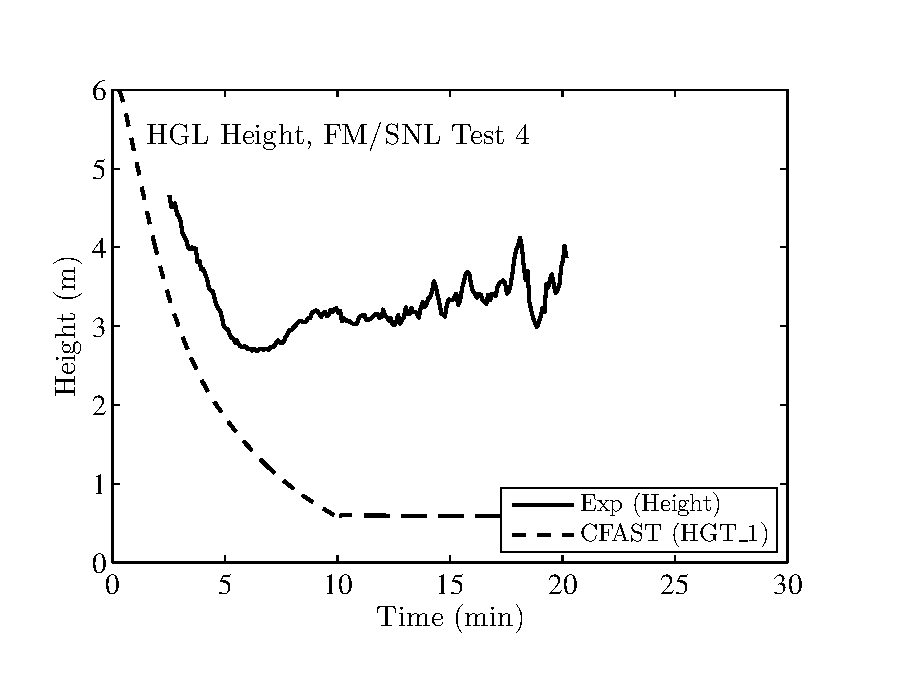
\includegraphics[width=2.6in]{FIGURES/FM_SNL/FM_SNL_04_HGL_Height} 
\end{tabular*}
\caption{Hot Gas Layer Temperature and Height for the FM/SNL Tests.} \label{fig:FM_SNL_HGL}
\end{figure}

\begin{figure}[p]
\begin{tabular*}{\textwidth}{l@{\extracolsep{\fill}}r}
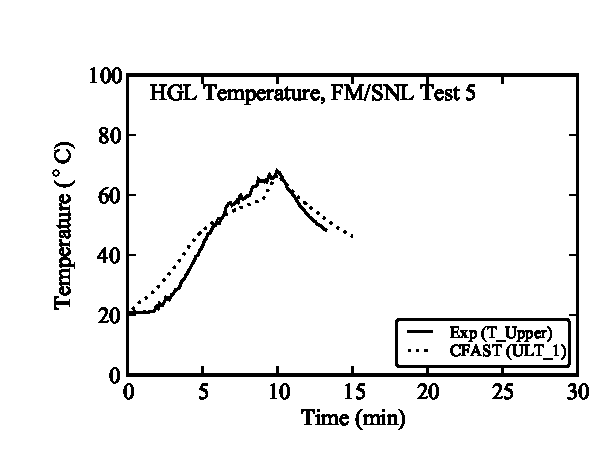
\includegraphics[width=2.6in]{FIGURES/FM_SNL/FM_SNL_05_HGL_Temp} &
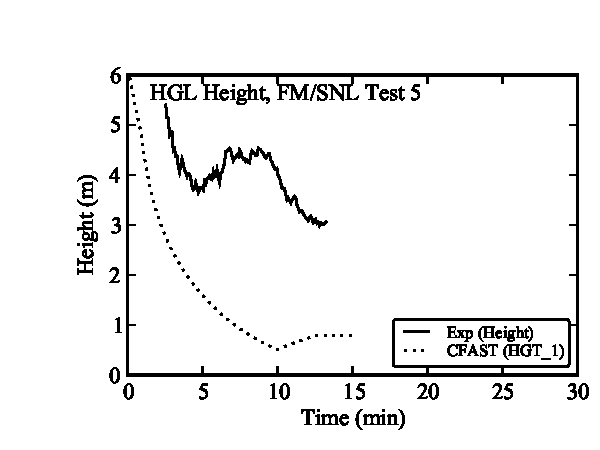
\includegraphics[width=2.6in]{FIGURES/FM_SNL/FM_SNL_05_HGL_Height} \\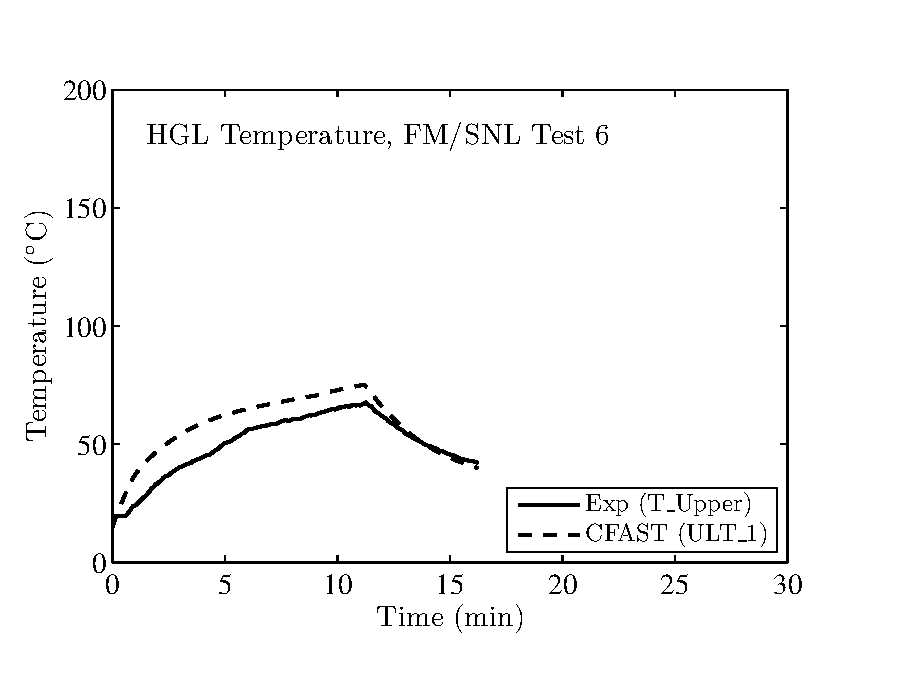
\includegraphics[width=2.6in]{FIGURES/FM_SNL/FM_SNL_06_HGL_Temp} &
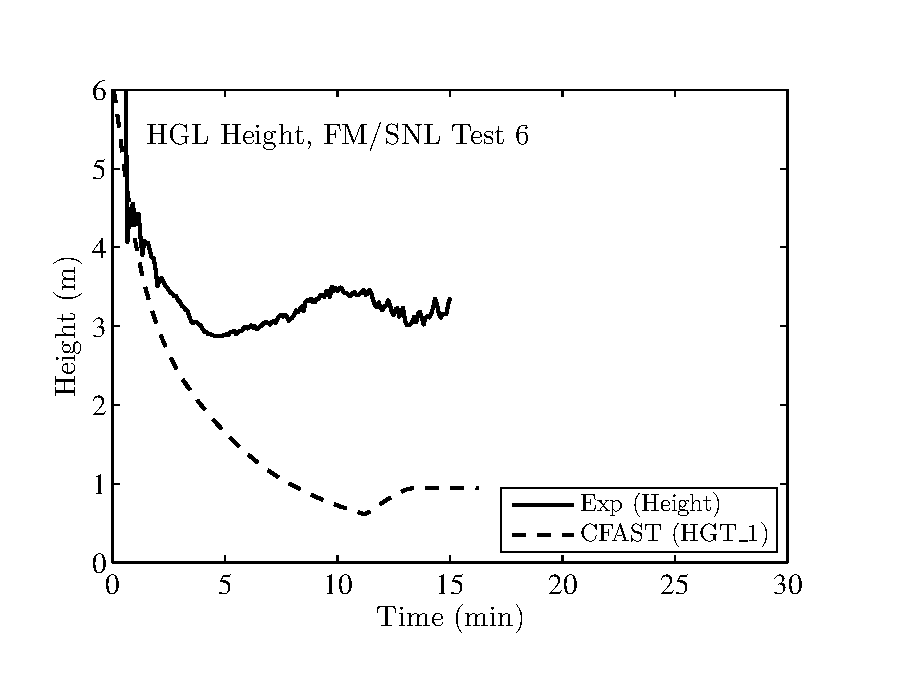
\includegraphics[width=2.6in]{FIGURES/FM_SNL/FM_SNL_06_HGL_Height} \\
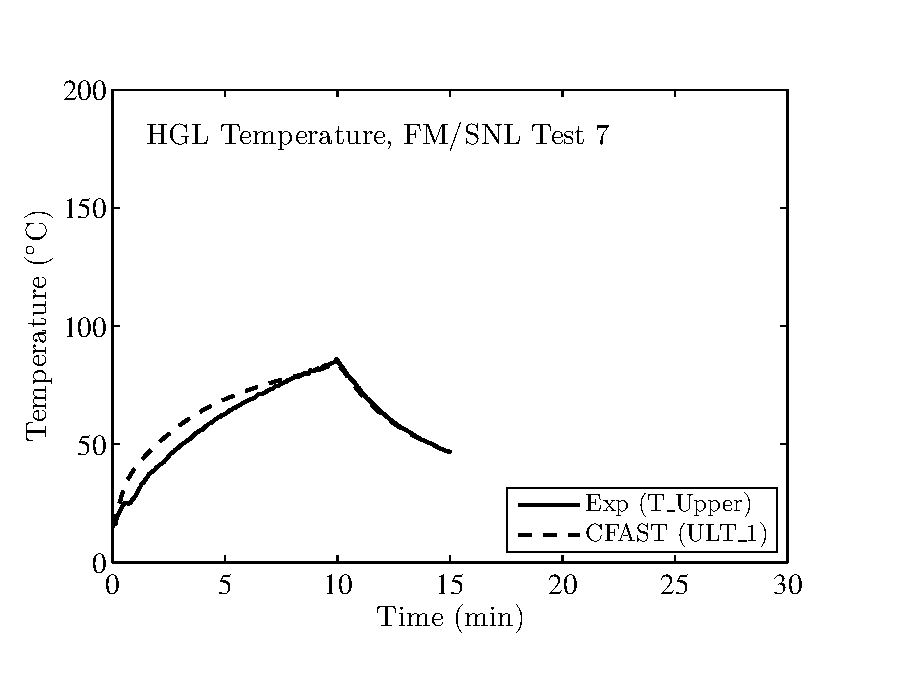
\includegraphics[width=2.6in]{FIGURES/FM_SNL/FM_SNL_07_HGL_Temp} &
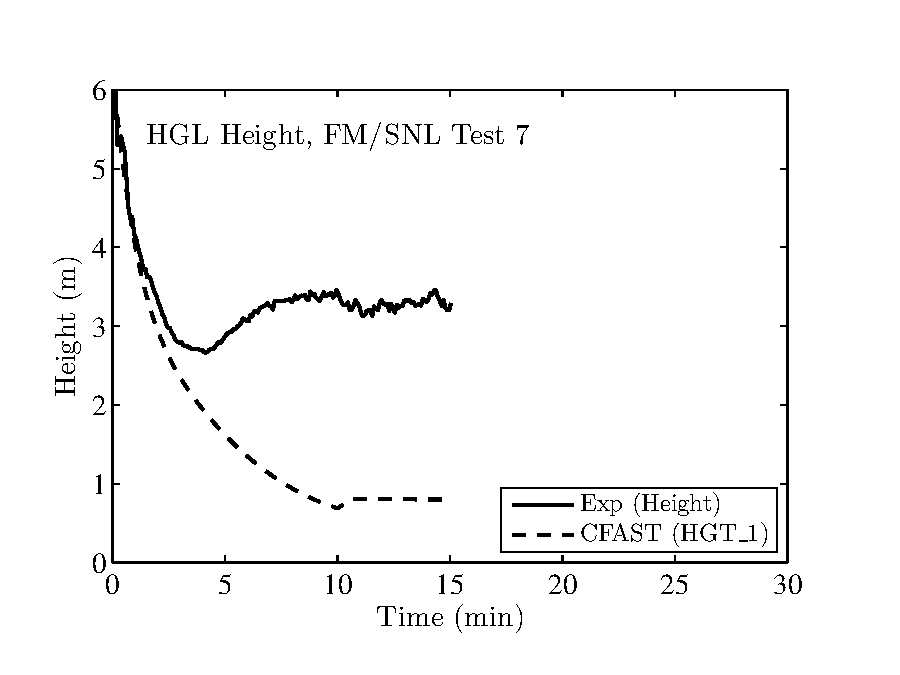
\includegraphics[width=2.6in]{FIGURES/FM_SNL/FM_SNL_07_HGL_Height} \\
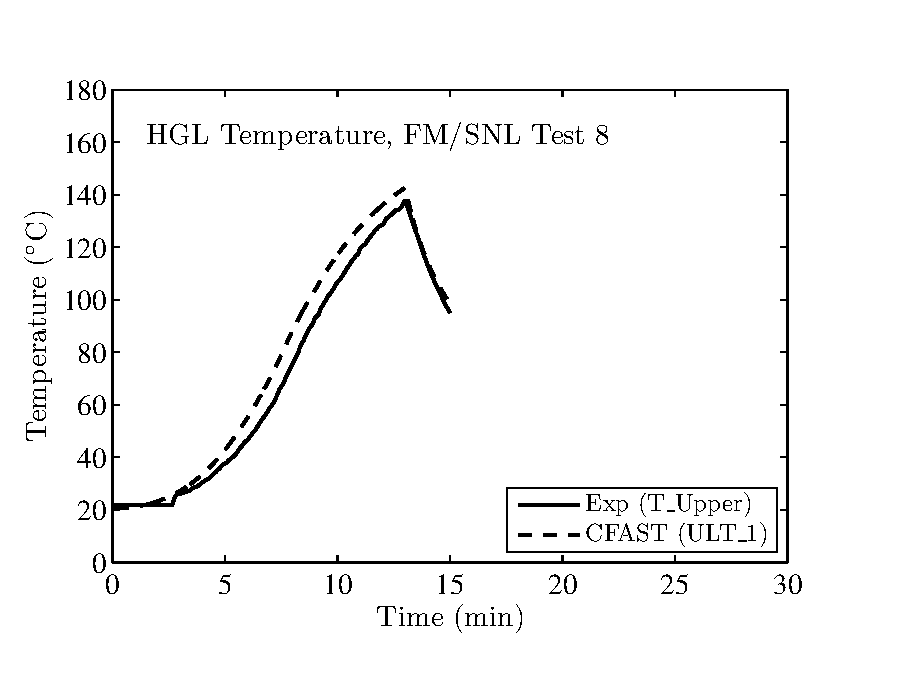
\includegraphics[width=2.6in]{FIGURES/FM_SNL/FM_SNL_08_HGL_Temp} &
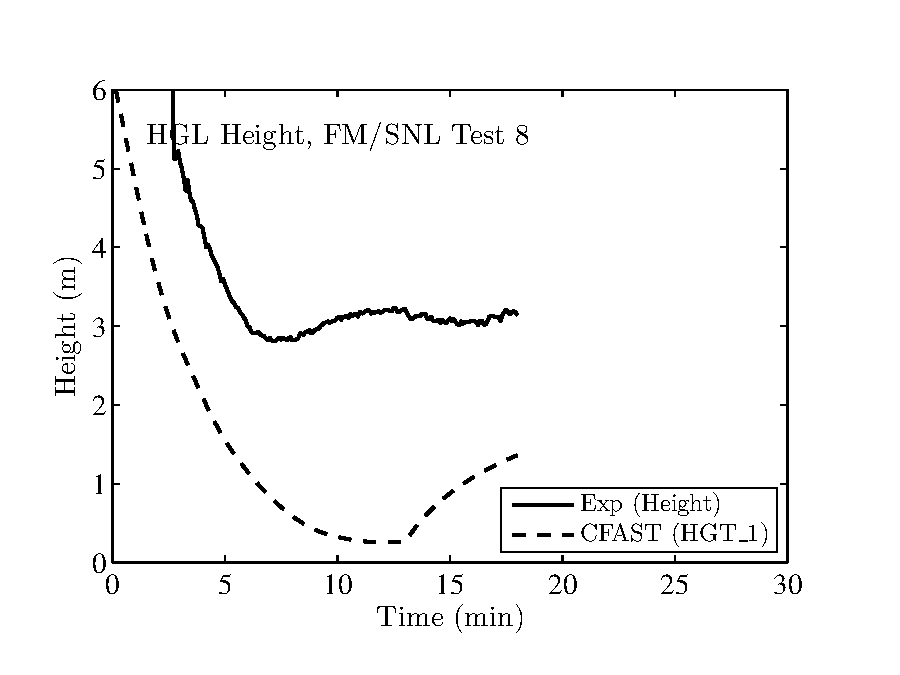
\includegraphics[width=2.6in]{FIGURES/FM_SNL/FM_SNL_08_HGL_Height}
\end{tabular*}
\caption{Hot Gas Layer Temperature and Height for the FM/SNL Tests.} \label{fig:FM_SNL_HGL}
\end{figure}

\begin{figure}[p]
\begin{tabular*}{\textwidth}{l@{\extracolsep{\fill}}r}
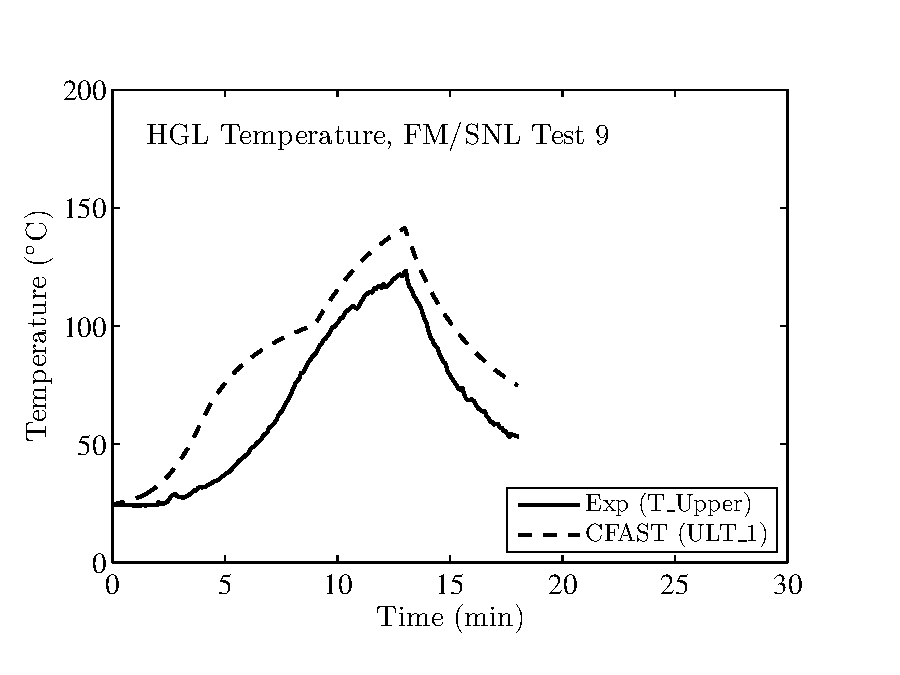
\includegraphics[width=2.6in]{FIGURES/FM_SNL/FM_SNL_09_HGL_Temp} &
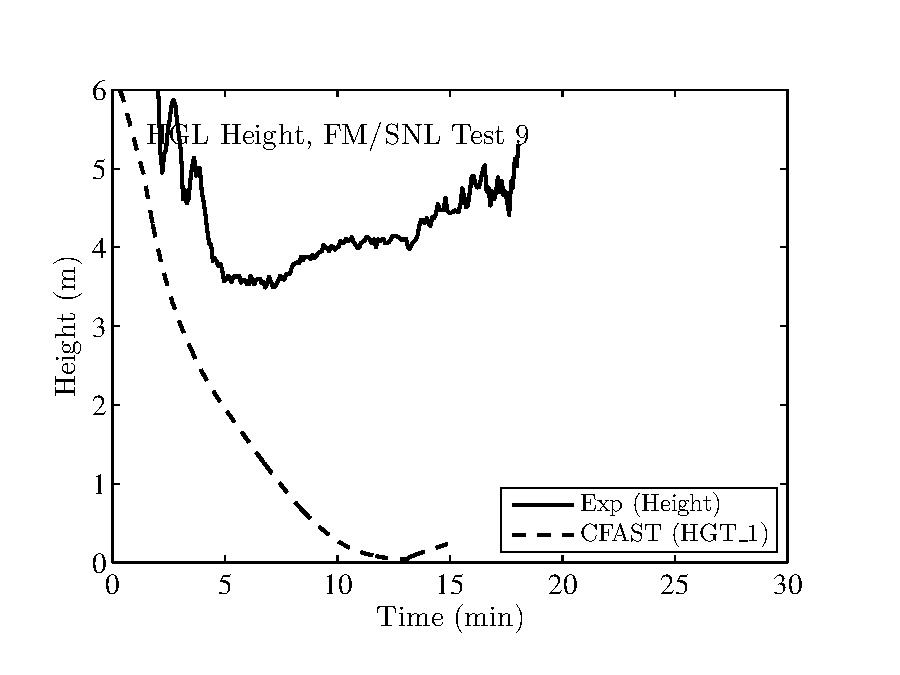
\includegraphics[width=2.6in]{FIGURES/FM_SNL/FM_SNL_09_HGL_Height} \\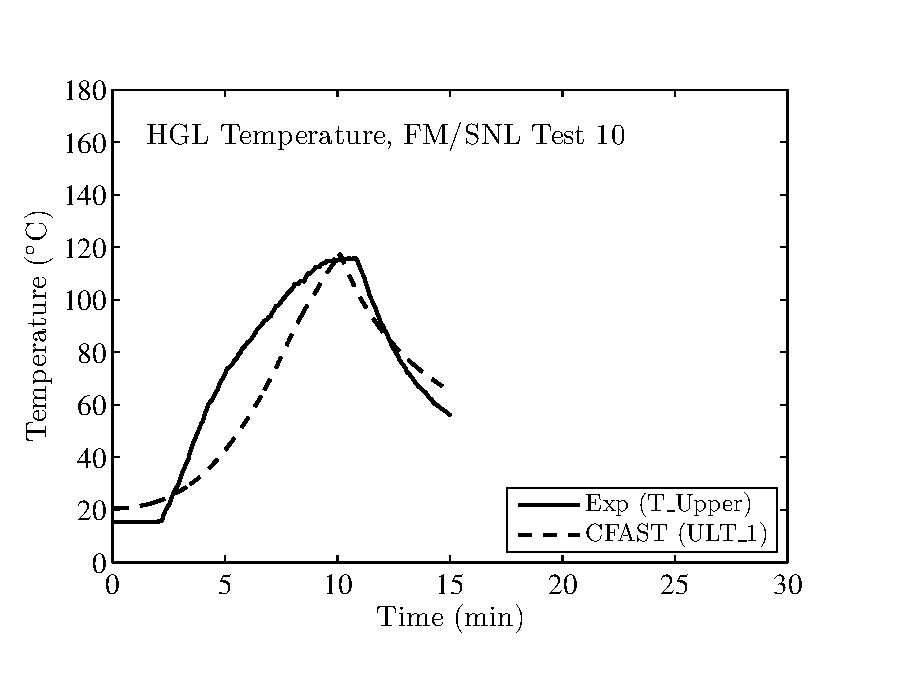
\includegraphics[width=2.6in]{FIGURES/FM_SNL/FM_SNL_10_HGL_Temp} &
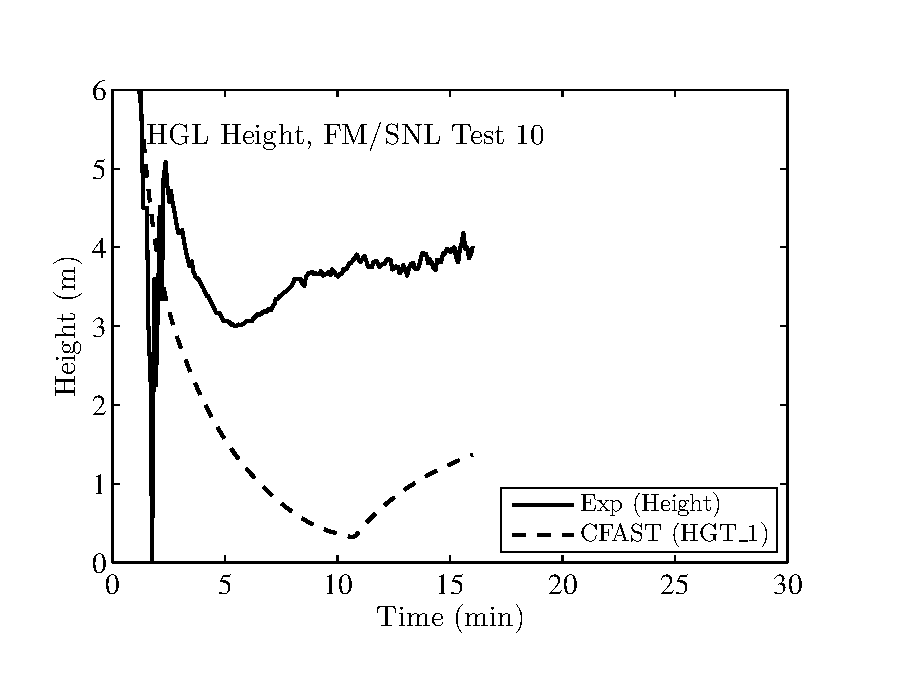
\includegraphics[width=2.6in]{FIGURES/FM_SNL/FM_SNL_10_HGL_Height} \\
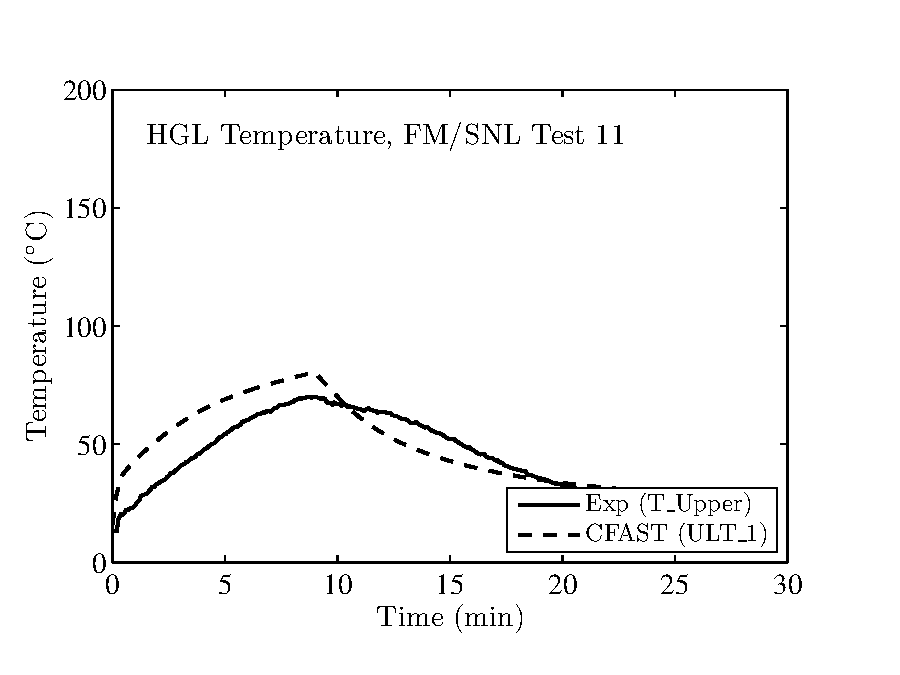
\includegraphics[width=2.6in]{FIGURES/FM_SNL/FM_SNL_11_HGL_Temp} &
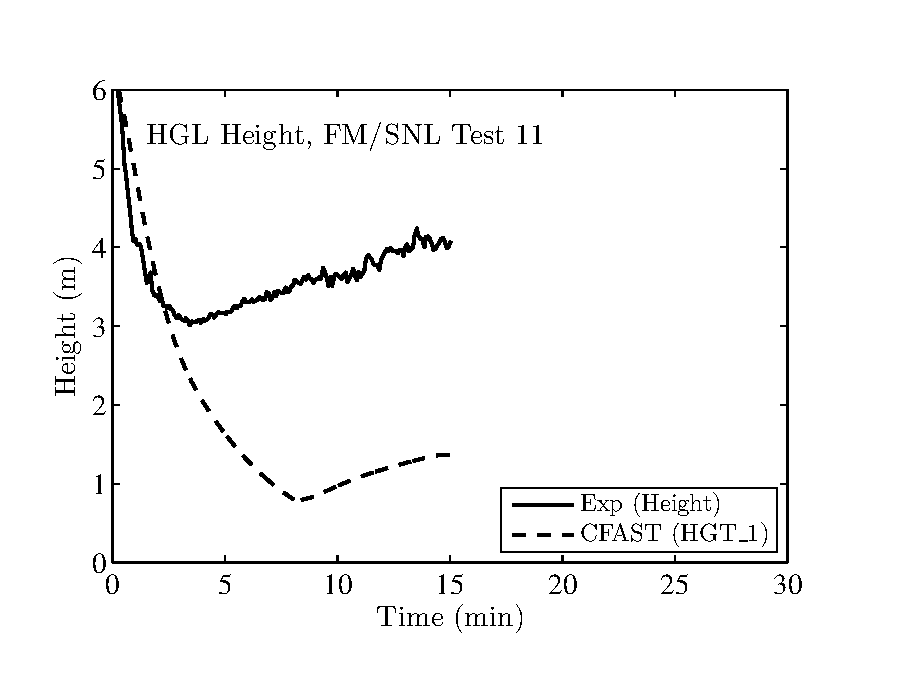
\includegraphics[width=2.6in]{FIGURES/FM_SNL/FM_SNL_11_HGL_Height} \\
\includegraphics[width=2.6in]{FIGURES/FM_SNL/FM_SNL_12_HGL_Temp} &
\includegraphics[width=2.6in]{FIGURES/FM_SNL/FM_SNL_12_HGL_Height}
\end{tabular*}
\caption{Hot Gas Layer Temperature and Height for the FM/SNL Tests.} \label{fig:FM_SNL_HGL}
\end{figure}

\begin{figure}[p]
\begin{tabular*}{\textwidth}{l@{\extracolsep{\fill}}r}
\includegraphics[width=2.6in]{FIGURES/FM_SNL/FM_SNL_13_HGL_Temp} &
\includegraphics[width=2.6in]{FIGURES/FM_SNL/FM_SNL_13_HGL_Height} \\
\includegraphics[width=2.6in]{FIGURES/FM_SNL/FM_SNL_14_HGL_Temp} &
\includegraphics[width=2.6in]{FIGURES/FM_SNL/FM_SNL_14_HGL_Height} \\
\includegraphics[width=2.6in]{FIGURES/FM_SNL/FM_SNL_15_HGL_Temp} &
\includegraphics[width=2.6in]{FIGURES/FM_SNL/FM_SNL_15_HGL_Height} \\
\includegraphics[width=2.6in]{FIGURES/FM_SNL/FM_SNL_16_HGL_Temp} &
\includegraphics[width=2.6in]{FIGURES/FM_SNL/FM_SNL_16_HGL_Height} 
\end{tabular*}
\caption{Hot Gas Layer Temperature and Height for the FM/SNL Tests.} \label{fig:FM_SNL_HGL}
\end{figure}

\begin{figure}[p]
\begin{tabular*}{\textwidth}{l@{\extracolsep{\fill}}r}
\includegraphics[width=2.6in]{FIGURES/FM_SNL/FM_SNL_17_HGL_Temp} &
\includegraphics[width=2.6in]{FIGURES/FM_SNL/FM_SNL_17_HGL_Height} \\
\includegraphics[width=2.6in]{FIGURES/FM_SNL/FM_SNL_21_HGL_Temp} &
\includegraphics[width=2.6in]{FIGURES/FM_SNL/FM_SNL_21_HGL_Height} \\
\includegraphics[width=2.6in]{FIGURES/FM_SNL/FM_SNL_22_HGL_Temp} &
\includegraphics[width=2.6in]{FIGURES/FM_SNL/FM_SNL_22_HGL_Height}
\end{tabular*}
\caption{Hot Gas Layer Temperature and Height for the FM/SNL Tests.} \label{fig:FM_SNL_HGL}
\end{figure}

\begin{figure}[p]
\begin{tabular*}{\textwidth}{l@{\extracolsep{\fill}}r}
\includegraphics[width=2.6in]{FIGURES/FM_SNL/FM_SNL_01_Plume_Temperature} &
\includegraphics[width=2.6in]{FIGURES/FM_SNL/FM_SNL_02_Plume_Temperature} \\
\includegraphics[width=2.6in]{FIGURES/FM_SNL/FM_SNL_03_Plume_Temperature} &
\includegraphics[width=2.6in]{FIGURES/FM_SNL/FM_SNL_04_Plume_Temperature} \\
\includegraphics[width=2.6in]{FIGURES/FM_SNL/FM_SNL_05_Plume_Temperature} &
\includegraphics[width=2.6in]{FIGURES/FM_SNL/FM_SNL_06_Plume_Temperature} \\
\includegraphics[width=2.6in]{FIGURES/FM_SNL/FM_SNL_07_Plume_Temperature} &
\includegraphics[width=2.6in]{FIGURES/FM_SNL/FM_SNL_08_Plume_Temperature} 
\end{tabular*}
\caption{Predicted Plume Centerline Temperature for the FM/SNL Tests.} \label{fig:FM_SNL_Plume}
\end{figure}

\begin{figure}[p]
\begin{tabular*}{\textwidth}{l@{\extracolsep{\fill}}r}
\includegraphics[width=2.6in]{FIGURES/FM_SNL/FM_SNL_09_Plume_Temperature} &
\includegraphics[width=2.6in]{FIGURES/FM_SNL/FM_SNL_10_Plume_Temperature} \\
\includegraphics[width=2.6in]{FIGURES/FM_SNL/FM_SNL_11_Plume_Temperature} &
\includegraphics[width=2.6in]{FIGURES/FM_SNL/FM_SNL_12_Plume_Temperature} \\
\includegraphics[width=2.6in]{FIGURES/FM_SNL/FM_SNL_13_Plume_Temperature} &
\includegraphics[width=2.6in]{FIGURES/FM_SNL/FM_SNL_14_Plume_Temperature} \\
\includegraphics[width=2.6in]{FIGURES/FM_SNL/FM_SNL_15_Plume_Temperature} &
\includegraphics[width=2.6in]{FIGURES/FM_SNL/FM_SNL_16_Plume_Temperature} 
\end{tabular*}
\caption{Predicted Plume Centerline Temperature for the FM/SNL Tests.} \label{fig:FM_SNL_Plume}
\end{figure}

\begin{figure}[p]
\begin{center}
\includegraphics[width=2.6in]{FIGURES/FM_SNL/FM_SNL_17_Plume_Temperature} \\
\includegraphics[width=2.6in]{FIGURES/FM_SNL/FM_SNL_21_Plume_Temperature} \\
\includegraphics[width=2.6in]{FIGURES/FM_SNL/FM_SNL_22_Plume_Temperature} 
\end{center}
\caption{Predicted Plume Centerline Temperature for the FM/SNL Tests.} \label{fig:FM_SNL_Plume}
\end{figure}

\begin{figure}[p]
\begin{tabular*}{\textwidth}{l@{\extracolsep{\fill}}r}
\includegraphics[width=2.6in]{FIGURES/FM_SNL/FM_SNL_01_Ceiling_Jet} &
\includegraphics[width=2.6in]{FIGURES/FM_SNL/FM_SNL_02_Ceiling_Jet} \\
\includegraphics[width=2.6in]{FIGURES/FM_SNL/FM_SNL_03_Ceiling_Jet} &
\includegraphics[width=2.6in]{FIGURES/FM_SNL/FM_SNL_04_Ceiling_Jet} \\
\includegraphics[width=2.6in]{FIGURES/FM_SNL/FM_SNL_05_Ceiling_Jet} &
\includegraphics[width=2.6in]{FIGURES/FM_SNL/FM_SNL_06_Ceiling_Jet} \\
\includegraphics[width=2.6in]{FIGURES/FM_SNL/FM_SNL_07_Ceiling_Jet} &
\includegraphics[width=2.6in]{FIGURES/FM_SNL/FM_SNL_08_Ceiling_Jet} 
\end{tabular*}
\caption{Predicted Plume Centerline Temperature for the FM/SNL Tests.} \label{fig:FM_SNL_Plume}
\end{figure}

\begin{figure}[p]
\begin{tabular*}{\textwidth}{l@{\extracolsep{\fill}}r}
\includegraphics[width=2.6in]{FIGURES/FM_SNL/FM_SNL_09_Ceiling_Jet} &
\includegraphics[width=2.6in]{FIGURES/FM_SNL/FM_SNL_10_Ceiling_Jet} \\
\includegraphics[width=2.6in]{FIGURES/FM_SNL/FM_SNL_11_Ceiling_Jet} &
\includegraphics[width=2.6in]{FIGURES/FM_SNL/FM_SNL_12_Ceiling_Jet} \\
\includegraphics[width=2.6in]{FIGURES/FM_SNL/FM_SNL_13_Ceiling_Jet} &
\includegraphics[width=2.6in]{FIGURES/FM_SNL/FM_SNL_14_Ceiling_Jet} \\
\includegraphics[width=2.6in]{FIGURES/FM_SNL/FM_SNL_15_Ceiling_Jet} &
\includegraphics[width=2.6in]{FIGURES/FM_SNL/FM_SNL_16_Ceiling_Jet} 
\end{tabular*}
\caption{Predicted Plume Centerline Temperature for the FM/SNL Tests.} \label{fig:FM_SNL_Plume}
\end{figure}

\begin{figure}[p]
\begin{center}
\includegraphics[width=2.6in]{FIGURES/FM_SNL/FM_SNL_17_Ceiling_Jet} \\
\includegraphics[width=2.6in]{FIGURES/FM_SNL/FM_SNL_21_Ceiling_Jet} \\
\includegraphics[width=2.6in]{FIGURES/FM_SNL/FM_SNL_22_Ceiling_Jet} 
\end{center}
\caption{Predicted Plume Centerline Temperature for the FM/SNL Tests.} \label{fig:FM_SNL_Plume}
\end{figure}

\clearpage

\section{iBMB Compartment Tests}

A series of small compartment kerosene pool fire experiments, conducted at the
Institut f�r Baustoffe, Massivbau und Brandschutz (iBMB) of Braunschweig University of
Technology in Germany in 2004 \cite{Klein-Helbetaling:2005}.  The results from Test 1 were
considered here.  These experiments involved relatively large fires in a relatively small (3.6 m x 3.6 m x 5.7 m) concrete enclosure. 

A second series of fire experiments in 2004, conducted under the International Collaborative Fire Model Project (ICFMP) involved realistically routed cable
trays inside the same concrete enclosure at iBMB \cite{Riese:2004}. The compartment was configured slightly differently with a ceiling height of 5.6 m. Six types of measurements conducted during the test series were used in the evaluation conducted here, including the HGL temperature and depth, oxygen gas concentration, the temperature of targets and compartment surfaces, and heat flux.


\begin{figure}[p]
\begin{tabular*}{\textwidth}{l@{\extracolsep{\fill}}r}
\includegraphics[width=2.6in]{FIGURES/iBMB/iBMB_Pool_HGL_Temp} &
\includegraphics[width=2.6in]{FIGURES/iBMB/iBMB_Pool_HGL_Height} \\
\includegraphics[width=2.6in]{FIGURES/iBMB/iBMB_Cable_HGL_Temp} &
\includegraphics[width=2.6in]{FIGURES/iBMB/iBMB_Cable_HGL_Height} 
\end{tabular*}
\caption{Predicted HGL Temperature and Height for the iBMB Single Compartment Tests.} \label{fig:iBMB_HGL}
\end{figure}

\begin{figure}[p]
\begin{tabular*}{\textwidth}{l@{\extracolsep{\fill}}r}
\includegraphics[width=2.6in]{FIGURES/iBMB/iBMB_Cable_Oxygen} &
\includegraphics[width=2.6in]{FIGURES/iBMB/iBMB_Cable_CO2} \\
\end{tabular*}
\caption{Predicted Oxygen and Carbon Dioxide for the iBMB Cable Test 5.} \label{fig:iBMB_Gases}
\end{figure}

\clearpage

\section{NBS Single Room Tests with Furniture}

These data describe a series of room fire tests using upholstered furniture items in a room of fixed size but with varying opening sizes and shapes \cite{Valid:Babrauskas_Flashover} conducted by the National Bureau of Standards (NBS, former name of NIST). It was selected for its well characterized and realistic fuel sources in a simple single-room geometry. In addition, the wide variation in opening size should provide challenges for current zone fire models. Peak fire size was about 2.9~MW with a total room volume of 21 m$^3$. A series of four single-room fire tests were conducted using upholstered furniture items for comparison with their free burning behavior, previously determined in a furniture calorimeter.  The experiments were conducted in a single room enclosure; ventilation to the room was provided by window openings of  varying sizes. The room was equipped with an instrumented exhaust collection system outside the window opening.  

A second similar test series also utilized a single-room fire test with furniture as the fire source \cite{Lee:1985}. It expanded upon the first data set by adding the phenomenon of wall burning. Peak fire size was about 7 MW. The room size was similar to the first test series.

\begin{figure}
\begin{tabular*}{\textwidth}{l@{\extracolsep{\fill}}r}
\includegraphics[width=2.6in]{FIGURES/NBS/1rfurn1_HGL_Temp} &
\includegraphics[width=2.6in]{FIGURES/NBS/1rfurn1_HGL_Height} \\
\includegraphics[width=2.6in]{FIGURES/NBS/1rfurn6_HGL_Temp} &
\includegraphics[width=2.6in]{FIGURES/NBS/1rfurn6_HGL_Height} \\
\includegraphics[width=2.6in]{FIGURES/NBS/1rwall1_HGL_Temp} &
\includegraphics[width=2.6in]{FIGURES/NBS/1rwall1_HGL_Height}\\
\includegraphics[width=2.6in]{FIGURES/NBS/1rwall2_HGL_Temp} &
\includegraphics[width=2.6in]{FIGURES/NBS/1rwall2_HGL_Height}
\end{tabular*}
\caption{Predicted HGL Temperature and Height for the NBS Single Compartment Tests.} \label{fig:1Room_HGL}
\end{figure}

\begin{figure}[p]
\begin{center}
\includegraphics[width=2.6in]{FIGURES/NBS/1rfurn1_Oxygen} \\
\includegraphics[width=2.6in]{FIGURES/NBS/1rfurn6_Oxygen} 
\end{center}
\caption{Predicted Oxygen Concentrationfor the NBS Single Compartment Tests.} \label{fig:1Room_Gases}
\end{figure}

\begin{figure}[p]
\begin{center}
\includegraphics[width=2.6in]{FIGURES/NBS/1rwall1_Pressure} \\
\includegraphics[width=2.6in]{FIGURES/NBS/1rwall2_Pressure} 
\end{center}
\caption{Predicted Compartment Pressure for the NBS Single Compartment Tests.} \label{fig:1Room_Pressure}
\end{figure}

\clearpage

\section{NBS Multi-Compartment Test Series}

The National Bureau of Standards (NBS, former name of NIST) Multi-Compartment Test Series consisted of 45 fire tests representing 9 different sets of conditions were conducted in a three-room suite.  The experiments were conducted in 1985 and are described in detail in reference \cite{Peacock:1988}.  The suite consisted of two relatively small rooms, connected via a relatively long corridor. Total volume of the structure was approximately 100 m$^2$. The fire source, a gas burner, was located against the rear wall of one of the small compartments . Fire tests of 100 kW, 300 kW and 500 kW were conducted. For the current  study, three 100 kW fire experiments have been used, including Test 100A from Set 1, Test 100O from Set 2, and Test 100Z from Set 4. For the NBS Multi-room series, Tests 100A, 100O and 100Z were selected for study, because they were constructively used in a previous validation study [\cite{EPRI}, and because these tests had  the steadiest values of measured heat release rate during the steady burning period. The selected data are also available in Reference \cite{EPRI}. 

\begin{figure}[p]
\begin{tabular*}{\textwidth}{l@{\extracolsep{\fill}}r}
\includegraphics[width=2.6in]{FIGURES/NBS/NBS_100A_Tree_1_HGL_Temp} &
\includegraphics[width=2.6in]{FIGURES/NBS/NBS_100A_Tree_1_HGL_Height} \\
\includegraphics[width=2.6in]{FIGURES/NBS/NBS_100A_Tree_4_HGL_Temp} &
\includegraphics[width=2.6in]{FIGURES/NBS/NBS_100A_Tree_4_HGL_Height} \\
\includegraphics[width=2.6in]{FIGURES/NBS/NBS_100A_Tree_5_HGL_Temp} &
\includegraphics[width=2.6in]{FIGURES/NBS/NBS_100A_Tree_5_HGL_Height}\\
\includegraphics[width=2.6in]{FIGURES/NBS/NBS_100A_Tree_6_HGL_Temp} &
\includegraphics[width=2.6in]{FIGURES/NBS/NBS_100A_Tree_6_HGL_Height}
\end{tabular*}
\caption{Hot Gas Layer Temperature and Height for the NBS Multi-Room Test 100A.} \label{fig:NBS_100A_HGL}
\end{figure}

\begin{figure}[p]
\begin{tabular*}{\textwidth}{l@{\extracolsep{\fill}}r}
\includegraphics[width=2.6in]{FIGURES/NBS/NBS_100O_Tree_1_HGL_Temp} &
\includegraphics[width=2.6in]{FIGURES/NBS/NBS_100O_Tree_1_HGL_Height} \\
\includegraphics[width=2.6in]{FIGURES/NBS/NBS_100O_Tree_4_HGL_Temp} &
\includegraphics[width=2.6in]{FIGURES/NBS/NBS_100O_Tree_4_HGL_Height} \\
\includegraphics[width=2.6in]{FIGURES/NBS/NBS_100O_Tree_5_HGL_Temp} &
\includegraphics[width=2.6in]{FIGURES/NBS/NBS_100O_Tree_5_HGL_Height}\\
\includegraphics[width=2.6in]{FIGURES/NBS/NBS_100O_Tree_6_HGL_Temp} &
\includegraphics[width=2.6in]{FIGURES/NBS/NBS_100O_Tree_6_HGL_Height}
\end{tabular*}
\caption{Hot Gas Layer Temperature and Height for the NBS Multi-Room Test 100O.} \label{fig:NBS_100O_HGL}
\end{figure}

\begin{figure}[p]
\begin{tabular*}{\textwidth}{l@{\extracolsep{\fill}}r}
\includegraphics[width=2.6in]{FIGURES/NBS/NBS_100Z_Tree_1_HGL_Temp} &
\includegraphics[width=2.6in]{FIGURES/NBS/NBS_100Z_Tree_1_HGL_Height} \\
\includegraphics[width=2.6in]{FIGURES/NBS/NBS_100Z_Tree_4_HGL_Temp} &
\includegraphics[width=2.6in]{FIGURES/NBS/NBS_100Z_Tree_4_HGL_Height} \\
\includegraphics[width=2.6in]{FIGURES/NBS/NBS_100Z_Tree_5_HGL_Temp} &
\includegraphics[width=2.6in]{FIGURES/NBS/NBS_100Z_Tree_5_HGL_Height}\\
\includegraphics[width=2.6in]{FIGURES/NBS/NBS_100Z_Tree_7_HGL_Temp} &
\includegraphics[width=2.6in]{FIGURES/NBS/NBS_100Z_Tree_7_HGL_Height}
\end{tabular*}
\caption{Hot Gas Layer Temperature and Height for the NBS Multi-Room Test 100Z.} \label{fig:NBS_100Z_HGL}
\end{figure}

\clearpage

\section{NIST Seven-story Hotel Tests}

By far the most complex test, this data set is part of  a series of full-scale experiments conducted to evaluate zoned smoke control systems, with and without stairwell pressurization \cite{Klote:1990}.  It was conducted in a seven story hotel with multiple rooms on each floor and a stairwell connecting all floors.  This data set was chosen because it would challenge the scope of most current fire models.  Measured temperatures and pressure differences between the rooms and floors of the building are extensive and consistent.  Peak fire size was 3 MW with a total building volume of 140~000 m$^3$. The hotel was a masonry structure consisting of two wings, one three stories and the other seven stories tall. The fires were set on the second floor of the seven-story wing. 

\begin{figure}[p]
\begin{center}
\includegraphics[width=2.6in]{FIGURES/NIST_PLAZA/Room_1_HGL_Temp} \\
\includegraphics[width=2.6in]{FIGURES/NIST_PLAZA/Room_2_HGL_Temp} \\
\includegraphics[width=2.6in]{FIGURES/NIST_PLAZA/Room_7_HGL_Temp}
\end{center}
\caption{Predicted HGL Temperature and Height for the Seven-Story Hotel Test 7.} \label{fig:NIST_PLAZA_HGL}
\end{figure}

\begin{figure}[p]
\begin{center}
\includegraphics[width=2.6in]{FIGURES/NIST_PLAZA/Room_2_Oxygen} \\
\includegraphics[width=2.6in]{FIGURES/NIST_PLAZA/Room_2_CO2} 
\end{center}
\caption{Predicted Oxygen and Carbon Dioxide for the Seven-Story Hotel Test 7.} \label{fig:NIST_PLAZA_HGL}
\end{figure}

\clearpage

\section{NIST/NRC Test Series}

These experiments, sponsored by the US NRC and conducted at NIST, consisted of 15 large-scale experiments performed in June 2003. All 15 tests were included in the validation study. The experiments are documented in Ref.~\cite{Hamins:2005}. The fire sizes ranged from 350 kW to 2.2 MW in a compartment with dimensions 21.7~m by 7.1~m by 3.8~m high, designed to represent a compartment in a nuclear power plant containing power and control cables. The room had one door and a simple mechanical ventilation system. Ventilation conditions, the fire size, and fire location were varied. Numerous measurements (approximately 350 per test) were made. 

\begin{figure}[p]
\begin{tabular*}{\textwidth}{l@{\extracolsep{\fill}}r}
\includegraphics[width=2.6in]{FIGURES/NIST_NRC/NIST_NRC_01_HGL_Temp} &
\includegraphics[width=2.6in]{FIGURES/NIST_NRC/NIST_NRC_01_HGL_Height} \\
\includegraphics[width=2.6in]{FIGURES/NIST_NRC/NIST_NRC_07_HGL_Temp} &
\includegraphics[width=2.6in]{FIGURES/NIST_NRC/NIST_NRC_07_HGL_Height} \\
\includegraphics[width=2.6in]{FIGURES/NIST_NRC/NIST_NRC_02_HGL_Temp} &
\includegraphics[width=2.6in]{FIGURES/NIST_NRC/NIST_NRC_02_HGL_Height} \\
\includegraphics[width=2.6in]{FIGURES/NIST_NRC/NIST_NRC_08_HGL_Temp} &
\includegraphics[width=2.6in]{FIGURES/NIST_NRC/NIST_NRC_08_HGL_Height}
\end{tabular*}
\caption{Predicted HGL Temperature and Height for the NIST/NRC Tests 1, 7, 2 and 8.} \label{fig:NIST_NRC_HGL_Closed_1}
\end{figure}

\begin{figure}[p]
\begin{tabular*}{\textwidth}{l@{\extracolsep{\fill}}r}
\includegraphics[width=2.6in]{FIGURES/NIST_NRC/NIST_NRC_04_HGL_Temp} &
\includegraphics[width=2.6in]{FIGURES/NIST_NRC/NIST_NRC_04_HGL_Height} \\
\includegraphics[width=2.6in]{FIGURES/NIST_NRC/NIST_NRC_10_HGL_Temp} &
\includegraphics[width=2.6in]{FIGURES/NIST_NRC/NIST_NRC_10_HGL_Height} \\
\includegraphics[width=2.6in]{FIGURES/NIST_NRC/NIST_NRC_13_HGL_Temp} &
\includegraphics[width=2.6in]{FIGURES/NIST_NRC/NIST_NRC_13_HGL_Height} \\
\includegraphics[width=2.6in]{FIGURES/NIST_NRC/NIST_NRC_16_HGL_Temp} &
\includegraphics[width=2.6in]{FIGURES/NIST_NRC/NIST_NRC_16_HGL_Height}
\end{tabular*}
\caption{Predicted HGL Temperature and Height for the NIST/NRC Tests 4, 10, 13 and 16.} \label{fig:NIST_NRC_HGL_Closed_2}
\end{figure}

\clearpage

\begin{figure}[p]
\begin{tabular*}{\textwidth}{l@{\extracolsep{\fill}}r}
\includegraphics[width=2.6in]{FIGURES/NIST_NRC/NIST_NRC_17_HGL_Temp} &
\includegraphics[width=2.6in]{FIGURES/NIST_NRC/NIST_NRC_17_HGL_Height} \\
\multicolumn{2}{c}{Open Door Tests to follow} \\
\includegraphics[width=2.6in]{FIGURES/NIST_NRC/NIST_NRC_03_HGL_Temp} &
\includegraphics[width=2.6in]{FIGURES/NIST_NRC/NIST_NRC_03_HGL_Height} \\
\includegraphics[width=2.6in]{FIGURES/NIST_NRC/NIST_NRC_09_HGL_Temp} &
\includegraphics[width=2.6in]{FIGURES/NIST_NRC/NIST_NRC_09_HGL_Height}
\end{tabular*}
\caption{Predicted HGL Temperature and Height for the NIST/NRC Tests 17, 3 and 9.} \label{fig:NIST_NRC_HGL_Open_1}
\end{figure}

\begin{figure}[p]
\begin{tabular*}{\textwidth}{l@{\extracolsep{\fill}}r}
\includegraphics[width=2.6in]{FIGURES/NIST_NRC/NIST_NRC_05_HGL_Temp} &
\includegraphics[width=2.6in]{FIGURES/NIST_NRC/NIST_NRC_05_HGL_Height} \\
\includegraphics[width=2.6in]{FIGURES/NIST_NRC/NIST_NRC_14_HGL_Temp} &
\includegraphics[width=2.6in]{FIGURES/NIST_NRC/NIST_NRC_14_HGL_Height} \\
\includegraphics[width=2.6in]{FIGURES/NIST_NRC/NIST_NRC_15_HGL_Temp} &
\includegraphics[width=2.6in]{FIGURES/NIST_NRC/NIST_NRC_15_HGL_Height} \\
\includegraphics[width=2.6in]{FIGURES/NIST_NRC/NIST_NRC_18_HGL_Temp} &
\includegraphics[width=2.6in]{FIGURES/NIST_NRC/NIST_NRC_18_HGL_Height}
\end{tabular*}
\caption{Predicted HGL Temperature and Height for the NIST/NRC Tests 5, 14, 15 and 18.} \label{fig:NIST_NRC_HGL_Open_2}
\end{figure}

\clearpage

\begin{figure}[p]
\begin{tabular*}{\textwidth}{l@{\extracolsep{\fill}}r}
\includegraphics[width=2.6in]{FIGURES/NIST_NRC/NIST_NRC_01_Ceiling_Jet} &
\includegraphics[width=2.6in]{FIGURES/NIST_NRC/NIST_NRC_07_Ceiling_Jet} \\
\includegraphics[width=2.6in]{FIGURES/NIST_NRC/NIST_NRC_02_Ceiling_Jet} &
\includegraphics[width=2.6in]{FIGURES/NIST_NRC/NIST_NRC_08_Ceiling_Jet} \\
\includegraphics[width=2.6in]{FIGURES/NIST_NRC/NIST_NRC_04_Ceiling_Jet} &
\includegraphics[width=2.6in]{FIGURES/NIST_NRC/NIST_NRC_10_Ceiling_Jet} \\
\includegraphics[width=2.6in]{FIGURES/NIST_NRC/NIST_NRC_13_Ceiling_Jet} &
\includegraphics[width=2.6in]{FIGURES/NIST_NRC/NIST_NRC_16_Ceiling_Jet}
\end{tabular*}
\caption{Ceiling Jet Temperature for the NIST/NRC Series, Closed Door Tests.}
\label{NIST_NRC_Jet_Closed}
\end{figure}

\begin{figure}[p]
\begin{tabular*}{\textwidth}{l@{\extracolsep{\fill}}r}
\includegraphics[width=2.6in]{FIGURES/NIST_NRC/NIST_NRC_17_Ceiling_Jet} &
 \\
\includegraphics[width=2.6in]{FIGURES/NIST_NRC/NIST_NRC_03_Ceiling_Jet} &
\includegraphics[width=2.6in]{FIGURES/NIST_NRC/NIST_NRC_09_Ceiling_Jet} \\
\includegraphics[width=2.6in]{FIGURES/NIST_NRC/NIST_NRC_05_Ceiling_Jet} &
\includegraphics[width=2.6in]{FIGURES/NIST_NRC/NIST_NRC_14_Ceiling_Jet} \\
\includegraphics[width=2.6in]{FIGURES/NIST_NRC/NIST_NRC_15_Ceiling_Jet} &
\includegraphics[width=2.6in]{FIGURES/NIST_NRC/NIST_NRC_18_Ceiling_Jet}
\end{tabular*}
\caption{Ceiling Jet Temperature for the NIST/NRC Series, Open Door Tests.}
\label{NIST_NRC_Jet_Open}
\end{figure}

\clearpage

\begin{figure}[p]
\begin{tabular*}{\textwidth}{l@{\extracolsep{\fill}}r}
\includegraphics[width=2.6in]{FIGURES/NIST_NRC/NIST_NRC_01_Oxygen} &
\includegraphics[width=2.6in]{FIGURES/NIST_NRC/NIST_NRC_01_CO2} \\
\includegraphics[width=2.6in]{FIGURES/NIST_NRC/NIST_NRC_07_Oxygen} &
\includegraphics[width=2.6in]{FIGURES/NIST_NRC/NIST_NRC_07_CO2} \\
\includegraphics[width=2.6in]{FIGURES/NIST_NRC/NIST_NRC_02_Oxygen} &
\includegraphics[width=2.6in]{FIGURES/NIST_NRC/NIST_NRC_02_CO2} \\
\includegraphics[width=2.6in]{FIGURES/NIST_NRC/NIST_NRC_08_Oxygen} &
\includegraphics[width=2.6in]{FIGURES/NIST_NRC/NIST_NRC_08_CO2}
\end{tabular*}
\caption{Predicted Oxygen and Carbon Dioxide for the NIST/NRC Tests 1, 7, 2 and 8.} \label{fig:NIST_NRC_Gases_Closed_1}
\end{figure}

\begin{figure}[p]
\begin{tabular*}{\textwidth}{l@{\extracolsep{\fill}}r}
\includegraphics[width=2.6in]{FIGURES/NIST_NRC/NIST_NRC_04_Oxygen} &
\includegraphics[width=2.6in]{FIGURES/NIST_NRC/NIST_NRC_04_CO2} \\
\includegraphics[width=2.6in]{FIGURES/NIST_NRC/NIST_NRC_10_Oxygen} &
\includegraphics[width=2.6in]{FIGURES/NIST_NRC/NIST_NRC_10_CO2} \\
\includegraphics[width=2.6in]{FIGURES/NIST_NRC/NIST_NRC_13_Oxygen} &
\includegraphics[width=2.6in]{FIGURES/NIST_NRC/NIST_NRC_13_CO2} \\
\includegraphics[width=2.6in]{FIGURES/NIST_NRC/NIST_NRC_16_Oxygen} &
\includegraphics[width=2.6in]{FIGURES/NIST_NRC/NIST_NRC_16_CO2}
\end{tabular*}
\caption{Predicted Oxygen and Carbon Dioxide for the NIST/NRC Tests 4, 10, 13 and 16.} \label{fig:NIST_NRC_Gases_Closed_2}
\end{figure}

\clearpage

\begin{figure}[p]
\begin{tabular*}{\textwidth}{l@{\extracolsep{\fill}}r}
\includegraphics[width=2.6in]{FIGURES/NIST_NRC/NIST_NRC_17_Oxygen} &
\includegraphics[width=2.6in]{FIGURES/NIST_NRC/NIST_NRC_17_CO2} \\
\multicolumn{2}{c}{Open Door Tests to follow} \\
\includegraphics[width=2.6in]{FIGURES/NIST_NRC/NIST_NRC_03_Oxygen} &
\includegraphics[width=2.6in]{FIGURES/NIST_NRC/NIST_NRC_03_CO2} \\
\includegraphics[width=2.6in]{FIGURES/NIST_NRC/NIST_NRC_09_Oxygen} &
\includegraphics[width=2.6in]{FIGURES/NIST_NRC/NIST_NRC_09_CO2}
\end{tabular*}
\caption{Predicted Oxygen and Carbon Dioxide for the NIST/NRC Tests 17, 3, and 9.} \label{fig:NIST_NRC_Gases_Open_1}
\end{figure}

\begin{figure}[p]
\begin{tabular*}{\textwidth}{l@{\extracolsep{\fill}}r}
\includegraphics[width=2.6in]{FIGURES/NIST_NRC/NIST_NRC_05_Oxygen} &
\includegraphics[width=2.6in]{FIGURES/NIST_NRC/NIST_NRC_05_CO2} \\
\includegraphics[width=2.6in]{FIGURES/NIST_NRC/NIST_NRC_14_Oxygen} &
\includegraphics[width=2.6in]{FIGURES/NIST_NRC/NIST_NRC_14_CO2} \\
\includegraphics[width=2.6in]{FIGURES/NIST_NRC/NIST_NRC_15_Oxygen} &
\includegraphics[width=2.6in]{FIGURES/NIST_NRC/NIST_NRC_15_CO2} \\
\includegraphics[width=2.6in]{FIGURES/NIST_NRC/NIST_NRC_18_Oxygen} &
\includegraphics[width=2.6in]{FIGURES/NIST_NRC/NIST_NRC_18_CO2}
\end{tabular*}
\caption{Predicted Oxygen and Carbon Dioxide for the NIST/NRC Tests 5, 14, 15 and 18.} \label{fig:NIST_NRC_Gases_Open_2}
\end{figure}

\clearpage

\begin{figure}[p]
\begin{tabular*}{\textwidth}{l@{\extracolsep{\fill}}r}
\includegraphics[width=2.6in]{FIGURES/NIST_NRC/NIST_NRC_01_Smoke} &
\includegraphics[width=2.6in]{FIGURES/NIST_NRC/NIST_NRC_07_Smoke} \\
\includegraphics[width=2.6in]{FIGURES/NIST_NRC/NIST_NRC_02_Smoke} &
\includegraphics[width=2.6in]{FIGURES/NIST_NRC/NIST_NRC_08_Smoke} \\
\includegraphics[width=2.6in]{FIGURES/NIST_NRC/NIST_NRC_04_Smoke} &
\includegraphics[width=2.6in]{FIGURES/NIST_NRC/NIST_NRC_10_Smoke} \\
\includegraphics[width=2.6in]{FIGURES/NIST_NRC/NIST_NRC_13_Smoke} &
\includegraphics[width=2.6in]{FIGURES/NIST_NRC/NIST_NRC_16_Smoke}
\end{tabular*}
\caption{Smoke Concentrationfor the NIST/NRC Series, Closed Door Tests.}
\label{NIST_NRC_Smoke_Closed}
\end{figure}

\begin{figure}[p]
\begin{tabular*}{\textwidth}{l@{\extracolsep{\fill}}r}
\includegraphics[width=2.6in]{FIGURES/NIST_NRC/NIST_NRC_17_Smoke} & \\
\includegraphics[width=2.6in]{FIGURES/NIST_NRC/NIST_NRC_03_Smoke} &
\includegraphics[width=2.6in]{FIGURES/NIST_NRC/NIST_NRC_09_Smoke} \\
\includegraphics[width=2.6in]{FIGURES/NIST_NRC/NIST_NRC_05_Smoke} &
\includegraphics[width=2.6in]{FIGURES/NIST_NRC/NIST_NRC_14_Smoke} \\
\includegraphics[width=2.6in]{FIGURES/NIST_NRC/NIST_NRC_15_Smoke} &
\includegraphics[width=2.6in]{FIGURES/NIST_NRC/NIST_NRC_18_Smoke}
\end{tabular*}
\caption{Smoke Concentrationfor the NIST/NRC Series, Open Door Tests.}
\label{NIST_NRC_Smoke_Open}
\end{figure}

\clearpage

\begin{figure}[p]
\begin{tabular*}{\textwidth}{l@{\extracolsep{\fill}}r}
\includegraphics[width=2.6in]{FIGURES/NIST_NRC/NIST_NRC_01_Pressure} &
\includegraphics[width=2.6in]{FIGURES/NIST_NRC/NIST_NRC_07_Pressure} \\
\includegraphics[width=2.6in]{FIGURES/NIST_NRC/NIST_NRC_02_Pressure} &
\includegraphics[width=2.6in]{FIGURES/NIST_NRC/NIST_NRC_08_Pressure} \\
\includegraphics[width=2.6in]{FIGURES/NIST_NRC/NIST_NRC_04_Pressure} &
\includegraphics[width=2.6in]{FIGURES/NIST_NRC/NIST_NRC_10_Pressure} \\
\includegraphics[width=2.6in]{FIGURES/NIST_NRC/NIST_NRC_13_Pressure} &
\includegraphics[width=2.6in]{FIGURES/NIST_NRC/NIST_NRC_16_Pressure}
\end{tabular*}
\caption{Compartment Pressures for the NIST/NRC Series, Closed Door Tests.}
\label{NIST_NRC_Pressure_Closed}
\end{figure}

\begin{figure}[p]
\begin{tabular*}{\textwidth}{l@{\extracolsep{\fill}}r}
\includegraphics[width=2.6in]{FIGURES/NIST_NRC/NIST_NRC_17_Pressure} &
   \\
\includegraphics[width=2.6in]{FIGURES/NIST_NRC/NIST_NRC_03_Pressure} &
\includegraphics[width=2.6in]{FIGURES/NIST_NRC/NIST_NRC_09_Pressure} \\
\includegraphics[width=2.6in]{FIGURES/NIST_NRC/NIST_NRC_05_Pressure} &
\includegraphics[width=2.6in]{FIGURES/NIST_NRC/NIST_NRC_14_Pressure} \\
\includegraphics[width=2.6in]{FIGURES/NIST_NRC/NIST_NRC_15_Pressure} &
\includegraphics[width=2.6in]{FIGURES/NIST_NRC/NIST_NRC_18_Pressure}
\end{tabular*}
\caption{Compartment Pressures for the NIST/NRC Series, Open Door Tests.}
\label{NIST_NRC_Pressure_Open}
\end{figure}

\clearpage

\begin{figure}[p]
\begin{tabular*}{\textwidth}{l@{\extracolsep{\fill}}r}
\includegraphics[width=2.6in]{FIGURES/NIST_NRC/NIST_NRC_01_Cable_B_Temp} &
\includegraphics[width=2.6in]{FIGURES/NIST_NRC/NIST_NRC_07_Cable_B_Temp} \\
\includegraphics[width=2.6in]{FIGURES/NIST_NRC/NIST_NRC_01_Cable_B_Flux} &
\includegraphics[width=2.6in]{FIGURES/NIST_NRC/NIST_NRC_07_Cable_B_Flux} 
\end{tabular*}
\caption{NIST/NRC Series, Cable B Temperature and Heat Flux, Replicate Tests 1 and 7.}
\label{NIST_NRC_B_1_and_7}
\end{figure}

\begin{figure}[p]
\begin{tabular*}{\textwidth}{l@{\extracolsep{\fill}}r}
\includegraphics[width=2.6in]{FIGURES/NIST_NRC/NIST_NRC_02_Cable_B_Temp} &
\includegraphics[width=2.6in]{FIGURES/NIST_NRC/NIST_NRC_08_Cable_B_Temp} \\
\includegraphics[width=2.6in]{FIGURES/NIST_NRC/NIST_NRC_02_Cable_B_Flux} &
\includegraphics[width=2.6in]{FIGURES/NIST_NRC/NIST_NRC_08_Cable_B_Flux} 
\end{tabular*}
\caption{NIST/NRC Series, Cable B Temperature and Heat Flux, Replicate Tests 2 and 8.}
\label{NIST_NRC_B_2_and_8}
\end{figure}

\clearpage

\begin{figure}[p]
\begin{tabular*}{\textwidth}{l@{\extracolsep{\fill}}r}
\includegraphics[width=2.6in]{FIGURES/NIST_NRC/NIST_NRC_04_Cable_B_Temp} &
\includegraphics[width=2.6in]{FIGURES/NIST_NRC/NIST_NRC_10_Cable_B_Temp} \\
\includegraphics[width=2.6in]{FIGURES/NIST_NRC/NIST_NRC_04_Cable_B_Flux} &
\includegraphics[width=2.6in]{FIGURES/NIST_NRC/NIST_NRC_10_Cable_B_Flux} 
\end{tabular*}
\caption{NIST/NRC Series, Cable B Temperature and Heat Flux, Replicate Tests 4 and 10.}
\label{NIST_NRC_B_4_and_10}
\end{figure}

\begin{figure}[p]
\begin{tabular*}{\textwidth}{l@{\extracolsep{\fill}}r}
\includegraphics[width=2.6in]{FIGURES/NIST_NRC/NIST_NRC_13_Cable_B_Temp} &
\includegraphics[width=2.6in]{FIGURES/NIST_NRC/NIST_NRC_16_Cable_B_Temp} \\
\includegraphics[width=2.6in]{FIGURES/NIST_NRC/NIST_NRC_13_Cable_B_Flux} &
\includegraphics[width=2.6in]{FIGURES/NIST_NRC/NIST_NRC_16_Cable_B_Flux} 
\end{tabular*}
\caption{NIST/NRC Series, Cable B Temperature and Heat Flux, Replicate Tests 13 and 16.}
\label{NIST_NRC_B_13_and_16}
\end{figure}

\clearpage

\begin{figure}[p]
\begin{tabular*}{\textwidth}{l@{\extracolsep{\fill}}r}
\includegraphics[width=2.6in]{FIGURES/NIST_NRC/NIST_NRC_03_Cable_B_Temp} &
\includegraphics[width=2.6in]{FIGURES/NIST_NRC/NIST_NRC_09_Cable_B_Temp} \\
\includegraphics[width=2.6in]{FIGURES/NIST_NRC/NIST_NRC_03_Cable_B_Flux} &
\includegraphics[width=2.6in]{FIGURES/NIST_NRC/NIST_NRC_09_Cable_B_Flux} 
\end{tabular*}
\caption{NIST/NRC Series, Cable B Temperature and Heat Flux, Replicate Tests 3 and 9.}
\label{NIST_NRC_B_3_and_9}
\end{figure}

\begin{figure}[p]
\begin{tabular*}{\textwidth}{l@{\extracolsep{\fill}}r}
\includegraphics[width=2.6in]{FIGURES/NIST_NRC/NIST_NRC_05_Cable_B_Temp} &
\includegraphics[width=2.6in]{FIGURES/NIST_NRC/NIST_NRC_14_Cable_B_Temp} \\
\includegraphics[width=2.6in]{FIGURES/NIST_NRC/NIST_NRC_05_Cable_B_Flux} &
\includegraphics[width=2.6in]{FIGURES/NIST_NRC/NIST_NRC_14_Cable_B_Flux} 
\end{tabular*}
\caption{NIST/NRC Series, Cable B Temperature and Heat Flux, Replicate Tests 5 and 14.}
\label{NIST_NRC_B_5_and_14}
\end{figure}

\clearpage

\begin{figure}[p]
\begin{tabular*}{\textwidth}{l@{\extracolsep{\fill}}r}
\includegraphics[width=2.6in]{FIGURES/NIST_NRC/NIST_NRC_15_Cable_B_Temp} &
\includegraphics[width=2.6in]{FIGURES/NIST_NRC/NIST_NRC_18_Cable_B_Temp} \\
\includegraphics[width=2.6in]{FIGURES/NIST_NRC/NIST_NRC_15_Cable_B_Flux} &
\includegraphics[width=2.6in]{FIGURES/NIST_NRC/NIST_NRC_18_Cable_B_Flux} 
\end{tabular*}
\caption{NIST/NRC Series, Cable B Temperature and Heat Flux, Replicate Tests 15 and 18.}
\label{NIST_NRC_B_15_and_18}
\end{figure}

\clearpage

\begin{figure}[p]
\begin{tabular*}{\textwidth}{l@{\extracolsep{\fill}}r}
\includegraphics[width=2.6in]{FIGURES/NIST_NRC/NIST_NRC_01_Cable_D_Temp} &
\includegraphics[width=2.6in]{FIGURES/NIST_NRC/NIST_NRC_07_Cable_D_Temp} \\
\includegraphics[width=2.6in]{FIGURES/NIST_NRC/NIST_NRC_01_Cable_D_Flux} &
\includegraphics[width=2.6in]{FIGURES/NIST_NRC/NIST_NRC_07_Cable_D_Flux} 
\end{tabular*}
\caption{NIST/NRC Series, Cable D Temperature and Heat Flux, Replicate Tests 1 and 7.}
\label{NIST_NRC_D_1_and_7}
\end{figure}

\begin{figure}[p]
\begin{tabular*}{\textwidth}{l@{\extracolsep{\fill}}r}
\includegraphics[width=2.6in]{FIGURES/NIST_NRC/NIST_NRC_02_Cable_D_Temp} &
\includegraphics[width=2.6in]{FIGURES/NIST_NRC/NIST_NRC_08_Cable_D_Temp} \\
\includegraphics[width=2.6in]{FIGURES/NIST_NRC/NIST_NRC_02_Cable_D_Flux} &
\includegraphics[width=2.6in]{FIGURES/NIST_NRC/NIST_NRC_08_Cable_D_Flux} 
\end{tabular*}
\caption{NIST/NRC Series, Cable D Temperature and Heat Flux, Replicate Tests 2 and 8.}
\label{NIST_NRC_D_2_and_8}
\end{figure}

\clearpage

\begin{figure}[p]
\begin{tabular*}{\textwidth}{l@{\extracolsep{\fill}}r}
\includegraphics[width=2.6in]{FIGURES/NIST_NRC/NIST_NRC_04_Cable_D_Temp} &
\includegraphics[width=2.6in]{FIGURES/NIST_NRC/NIST_NRC_10_Cable_D_Temp} \\
\includegraphics[width=2.6in]{FIGURES/NIST_NRC/NIST_NRC_04_Cable_D_Flux} &
\includegraphics[width=2.6in]{FIGURES/NIST_NRC/NIST_NRC_10_Cable_D_Flux} 
\end{tabular*}
\caption{NIST/NRC Series, Cable D Temperature and Heat Flux, Replicate Tests 4 and 10.}
\label{NIST_NRC_D_4_and_10}
\end{figure}

\begin{figure}[p]
\begin{tabular*}{\textwidth}{l@{\extracolsep{\fill}}r}
\includegraphics[width=2.6in]{FIGURES/NIST_NRC/NIST_NRC_13_Cable_D_Temp} &
\includegraphics[width=2.6in]{FIGURES/NIST_NRC/NIST_NRC_16_Cable_D_Temp} \\
\includegraphics[width=2.6in]{FIGURES/NIST_NRC/NIST_NRC_13_Cable_D_Flux} &
\includegraphics[width=2.6in]{FIGURES/NIST_NRC/NIST_NRC_16_Cable_D_Flux} 
\end{tabular*}
\caption{NIST/NRC Series, Cable D Temperature and Heat Flux, Replicate Tests 13 and 16.}
\label{NIST_NRC_D_13_and_16}
\end{figure}

\clearpage

\begin{figure}[p]
\begin{tabular*}{\textwidth}{l@{\extracolsep{\fill}}r}
\includegraphics[width=2.6in]{FIGURES/NIST_NRC/NIST_NRC_03_Cable_D_Temp} &
\includegraphics[width=2.6in]{FIGURES/NIST_NRC/NIST_NRC_09_Cable_D_Temp} \\
\includegraphics[width=2.6in]{FIGURES/NIST_NRC/NIST_NRC_03_Cable_D_Flux} &
\includegraphics[width=2.6in]{FIGURES/NIST_NRC/NIST_NRC_09_Cable_D_Flux} 
\end{tabular*}
\caption{NIST/NRC Series, Cable D Temperature and Heat Flux, Replicate Tests 3 and 9.}
\label{NIST_NRC_D_3_and_9}
\end{figure}

\begin{figure}[p]
\begin{tabular*}{\textwidth}{l@{\extracolsep{\fill}}r}
\includegraphics[width=2.6in]{FIGURES/NIST_NRC/NIST_NRC_05_Cable_D_Temp} &
\includegraphics[width=2.6in]{FIGURES/NIST_NRC/NIST_NRC_14_Cable_D_Temp} \\
\includegraphics[width=2.6in]{FIGURES/NIST_NRC/NIST_NRC_05_Cable_D_Flux} &
\includegraphics[width=2.6in]{FIGURES/NIST_NRC/NIST_NRC_14_Cable_D_Flux} 
\end{tabular*}
\caption{NIST/NRC Series, Cable D Temperature and Heat Flux, Replicate Tests 5 and 14.}
\label{NIST_NRC_D_5_and_14}
\end{figure}

\clearpage

\begin{figure}[p]
\begin{tabular*}{\textwidth}{l@{\extracolsep{\fill}}r}
\includegraphics[width=2.6in]{FIGURES/NIST_NRC/NIST_NRC_15_Cable_D_Temp} &
\includegraphics[width=2.6in]{FIGURES/NIST_NRC/NIST_NRC_18_Cable_D_Temp} \\
\includegraphics[width=2.6in]{FIGURES/NIST_NRC/NIST_NRC_15_Cable_D_Flux} &
\includegraphics[width=2.6in]{FIGURES/NIST_NRC/NIST_NRC_18_Cable_D_Flux} 
\end{tabular*}
\caption{NIST/NRC Series, Cable D Temperature and Heat Flux, Replicate Tests 15 and 18.}
\label{NIST_NRC_D_15_and_18}
\end{figure}

\clearpage

\begin{figure}[p]
\begin{tabular*}{\textwidth}{l@{\extracolsep{\fill}}r}
\includegraphics[width=2.6in]{FIGURES/NIST_NRC/NIST_NRC_01_Cable_F_Temp} &
\includegraphics[width=2.6in]{FIGURES/NIST_NRC/NIST_NRC_07_Cable_F_Temp} \\
\includegraphics[width=2.6in]{FIGURES/NIST_NRC/NIST_NRC_01_Cable_F_Flux} &
\includegraphics[width=2.6in]{FIGURES/NIST_NRC/NIST_NRC_07_Cable_F_Flux} 
\end{tabular*}
\caption{NIST/NRC Series, Cable F Temperature and Heat Flux, Replicate Tests 1 and 7.}
\label{NIST_NRC_F_1_and_7}
\end{figure}

\begin{figure}[p]
\begin{tabular*}{\textwidth}{l@{\extracolsep{\fill}}r}
\includegraphics[width=2.6in]{FIGURES/NIST_NRC/NIST_NRC_02_Cable_F_Temp} &
\includegraphics[width=2.6in]{FIGURES/NIST_NRC/NIST_NRC_08_Cable_F_Temp} \\
\includegraphics[width=2.6in]{FIGURES/NIST_NRC/NIST_NRC_02_Cable_F_Flux} &
\includegraphics[width=2.6in]{FIGURES/NIST_NRC/NIST_NRC_08_Cable_F_Flux} 
\end{tabular*}
\caption{NIST/NRC Series, Cable F Temperature and Heat Flux, Replicate Tests 2 and 8.}
\label{NIST_NRC_F_2_and_8}
\end{figure}

\clearpage

\begin{figure}[p]
\begin{tabular*}{\textwidth}{l@{\extracolsep{\fill}}r}
\includegraphics[width=2.6in]{FIGURES/NIST_NRC/NIST_NRC_04_Cable_F_Temp} &
\includegraphics[width=2.6in]{FIGURES/NIST_NRC/NIST_NRC_10_Cable_F_Temp} \\
\includegraphics[width=2.6in]{FIGURES/NIST_NRC/NIST_NRC_04_Cable_F_Flux} &
\includegraphics[width=2.6in]{FIGURES/NIST_NRC/NIST_NRC_10_Cable_F_Flux} 
\end{tabular*}
\caption{NIST/NRC Series, Cable F Temperature and Heat Flux, Replicate Tests 4 and 10.}
\label{NIST_NRC_F_4_and_10}
\end{figure}

\begin{figure}[p]
\begin{tabular*}{\textwidth}{l@{\extracolsep{\fill}}r}
\includegraphics[width=2.6in]{FIGURES/NIST_NRC/NIST_NRC_13_Cable_F_Temp} &
\includegraphics[width=2.6in]{FIGURES/NIST_NRC/NIST_NRC_16_Cable_F_Temp} \\
\includegraphics[width=2.6in]{FIGURES/NIST_NRC/NIST_NRC_13_Cable_F_Flux} &
\includegraphics[width=2.6in]{FIGURES/NIST_NRC/NIST_NRC_16_Cable_F_Flux} 
\end{tabular*}
\caption{NIST/NRC Series, Cable F Temperature and Heat Flux, Replicate Tests 13 and 16.}
\label{NIST_NRC_F_13_and_16}
\end{figure}

\clearpage

\begin{figure}[p]
\begin{tabular*}{\textwidth}{l@{\extracolsep{\fill}}r}
\includegraphics[width=2.6in]{FIGURES/NIST_NRC/NIST_NRC_03_Cable_F_Temp} &
\includegraphics[width=2.6in]{FIGURES/NIST_NRC/NIST_NRC_09_Cable_F_Temp} \\
\includegraphics[width=2.6in]{FIGURES/NIST_NRC/NIST_NRC_03_Cable_F_Flux} &
\includegraphics[width=2.6in]{FIGURES/NIST_NRC/NIST_NRC_09_Cable_F_Flux} 
\end{tabular*}
\caption{NIST/NRC Series, Cable F Temperature and Heat Flux, Replicate Tests 3 and 9.}
\label{NIST_NRC_F_3_and_9}
\end{figure}

\begin{figure}[p]
\begin{tabular*}{\textwidth}{l@{\extracolsep{\fill}}r}
\includegraphics[width=2.6in]{FIGURES/NIST_NRC/NIST_NRC_05_Cable_F_Temp} &
\includegraphics[width=2.6in]{FIGURES/NIST_NRC/NIST_NRC_14_Cable_F_Temp} \\
\includegraphics[width=2.6in]{FIGURES/NIST_NRC/NIST_NRC_05_Cable_F_Flux} &
\includegraphics[width=2.6in]{FIGURES/NIST_NRC/NIST_NRC_14_Cable_F_Flux} 
\end{tabular*}
\caption{NIST/NRC Series, Cable F Temperature and Heat Flux, Replicate Tests 5 and 14.}
\label{NIST_NRC_F_5_and_14}
\end{figure}

\clearpage

\begin{figure}[p]
\begin{tabular*}{\textwidth}{l@{\extracolsep{\fill}}r}
\includegraphics[width=2.6in]{FIGURES/NIST_NRC/NIST_NRC_15_Cable_F_Temp} &
\includegraphics[width=2.6in]{FIGURES/NIST_NRC/NIST_NRC_18_Cable_F_Temp} \\
\includegraphics[width=2.6in]{FIGURES/NIST_NRC/NIST_NRC_15_Cable_F_Flux} &
\includegraphics[width=2.6in]{FIGURES/NIST_NRC/NIST_NRC_18_Cable_F_Flux} 
\end{tabular*}
\caption{NIST/NRC Series, Cable F Temperature and Heat Flux, Replicate Tests 15 and 18.}
\label{NIST_NRC_F_15_and_18}
\end{figure}

\clearpage

\begin{figure}[p]
\begin{tabular*}{\textwidth}{l@{\extracolsep{\fill}}r}
\includegraphics[width=2.6in]{FIGURES/NIST_NRC/NIST_NRC_01_Cable_G_Temp} &
\includegraphics[width=2.6in]{FIGURES/NIST_NRC/NIST_NRC_07_Cable_G_Temp} \\
\includegraphics[width=2.6in]{FIGURES/NIST_NRC/NIST_NRC_01_Cable_G_Flux} &
\includegraphics[width=2.6in]{FIGURES/NIST_NRC/NIST_NRC_07_Cable_G_Flux} 
\end{tabular*}
\caption{NIST/NRC Series, Cable G Temperature and Heat Flux, Replicate Tests 1 and 7.}
\label{NIST_NRC_G_1_and_7}
\end{figure}

\begin{figure}[p]
\begin{tabular*}{\textwidth}{l@{\extracolsep{\fill}}r}
\includegraphics[width=2.6in]{FIGURES/NIST_NRC/NIST_NRC_02_Cable_G_Temp} &
\includegraphics[width=2.6in]{FIGURES/NIST_NRC/NIST_NRC_08_Cable_G_Temp} \\
\includegraphics[width=2.6in]{FIGURES/NIST_NRC/NIST_NRC_02_Cable_G_Flux} &
\includegraphics[width=2.6in]{FIGURES/NIST_NRC/NIST_NRC_08_Cable_G_Flux} 
\end{tabular*}
\caption{NIST/NRC Series, Cable G Temperature and Heat Flux, Replicate Tests 2 and 8.}
\label{NIST_NRC_G_2_and_8}
\end{figure}

\clearpage

\begin{figure}[p]
\begin{tabular*}{\textwidth}{l@{\extracolsep{\fill}}r}
\includegraphics[width=2.6in]{FIGURES/NIST_NRC/NIST_NRC_04_Cable_G_Temp} &
\includegraphics[width=2.6in]{FIGURES/NIST_NRC/NIST_NRC_10_Cable_G_Temp} \\
\includegraphics[width=2.6in]{FIGURES/NIST_NRC/NIST_NRC_04_Cable_G_Flux} &
\includegraphics[width=2.6in]{FIGURES/NIST_NRC/NIST_NRC_10_Cable_G_Flux} 
\end{tabular*}
\caption{NIST/NRC Series, Cable G Temperature and Heat Flux, Replicate Tests 4 and 10.}
\label{NIST_NRC_G_4_and_10}
\end{figure}

\begin{figure}[p]
\begin{tabular*}{\textwidth}{l@{\extracolsep{\fill}}r}
\includegraphics[width=2.6in]{FIGURES/NIST_NRC/NIST_NRC_13_Cable_G_Temp} &
\includegraphics[width=2.6in]{FIGURES/NIST_NRC/NIST_NRC_16_Cable_G_Temp} \\
\includegraphics[width=2.6in]{FIGURES/NIST_NRC/NIST_NRC_13_Cable_G_Flux} &
\includegraphics[width=2.6in]{FIGURES/NIST_NRC/NIST_NRC_16_Cable_G_Flux} 
\end{tabular*}
\caption{NIST/NRC Series, Cable G Temperature and Heat Flux, Replicate Tests 13 and 16.}
\label{NIST_NRC_G_13_and_16}
\end{figure}

\clearpage

\begin{figure}[p]
\begin{tabular*}{\textwidth}{l@{\extracolsep{\fill}}r}
\includegraphics[width=2.6in]{FIGURES/NIST_NRC/NIST_NRC_03_Cable_G_Temp} &
\includegraphics[width=2.6in]{FIGURES/NIST_NRC/NIST_NRC_09_Cable_G_Temp} \\
\includegraphics[width=2.6in]{FIGURES/NIST_NRC/NIST_NRC_03_Cable_G_Flux} &
\includegraphics[width=2.6in]{FIGURES/NIST_NRC/NIST_NRC_09_Cable_G_Flux} 
\end{tabular*}
\caption{NIST/NRC Series, Cable G Temperature and Heat Flux, Replicate Tests 3 and 9.}
\label{NIST_NRC_G_3_and_9}
\end{figure}

\begin{figure}[p]
\begin{tabular*}{\textwidth}{l@{\extracolsep{\fill}}r}
\includegraphics[width=2.6in]{FIGURES/NIST_NRC/NIST_NRC_05_Cable_G_Temp} &
\includegraphics[width=2.6in]{FIGURES/NIST_NRC/NIST_NRC_14_Cable_G_Temp} \\
\includegraphics[width=2.6in]{FIGURES/NIST_NRC/NIST_NRC_05_Cable_G_Flux} &
\includegraphics[width=2.6in]{FIGURES/NIST_NRC/NIST_NRC_14_Cable_G_Flux} 
\end{tabular*}
\caption{NIST/NRC Series, Cable G Temperature and Heat Flux, Replicate Tests 5 and 14.}
\label{NIST_NRC_G_5_and_14}
\end{figure}

\clearpage

\begin{figure}[p]
\begin{tabular*}{\textwidth}{l@{\extracolsep{\fill}}r}
\includegraphics[width=2.6in]{FIGURES/NIST_NRC/NIST_NRC_15_Cable_G_Temp} &
\includegraphics[width=2.6in]{FIGURES/NIST_NRC/NIST_NRC_18_Cable_G_Temp} \\
\includegraphics[width=2.6in]{FIGURES/NIST_NRC/NIST_NRC_15_Cable_G_Flux} &
\includegraphics[width=2.6in]{FIGURES/NIST_NRC/NIST_NRC_18_Cable_G_Flux} 
\end{tabular*}
\caption{NIST/NRC Series, Cable G Temperature and Heat Flux, Replicate Tests 15 and 18.}
\label{NIST_NRC_G_15_and_18}
\end{figure}

\clearpage

\begin{figure}[p]
\begin{tabular*}{\textwidth}{l@{\extracolsep{\fill}}r}
\includegraphics[width=2.6in]{FIGURES/NIST_NRC/NIST_NRC_01_Long_Wall_Temp} &
\includegraphics[width=2.6in]{FIGURES/NIST_NRC/NIST_NRC_07_Long_Wall_Temp} \\
\includegraphics[width=2.6in]{FIGURES/NIST_NRC/NIST_NRC_01_Long_Wall_Flux} &
\includegraphics[width=2.6in]{FIGURES/NIST_NRC/NIST_NRC_07_Long_Wall_Flux} 
\end{tabular*}
\caption{NIST/NRC Series, Long Wall Temperature and Heat Flux, Replicate Tests 1 and 7.}
\label{NIST_NRCLong_Wall_1_and_7}
\end{figure}

\begin{figure}[p]
\begin{tabular*}{\textwidth}{l@{\extracolsep{\fill}}r}
\includegraphics[width=2.6in]{FIGURES/NIST_NRC/NIST_NRC_02_Long_Wall_Temp} &
\includegraphics[width=2.6in]{FIGURES/NIST_NRC/NIST_NRC_08_Long_Wall_Temp} \\
\includegraphics[width=2.6in]{FIGURES/NIST_NRC/NIST_NRC_02_Long_Wall_Flux} &
\includegraphics[width=2.6in]{FIGURES/NIST_NRC/NIST_NRC_08_Long_Wall_Flux} 
\end{tabular*}
\caption{NIST/NRC Series, Long Wall Temperature and Heat Flux, Replicate Tests 2 and 8.}
\label{NIST_NRCLong_Wall_2_and_8}
\end{figure}

\clearpage

\begin{figure}[p]
\begin{tabular*}{\textwidth}{l@{\extracolsep{\fill}}r}
\includegraphics[width=2.6in]{FIGURES/NIST_NRC/NIST_NRC_04_Long_Wall_Temp} &
\includegraphics[width=2.6in]{FIGURES/NIST_NRC/NIST_NRC_10_Long_Wall_Temp} \\
\includegraphics[width=2.6in]{FIGURES/NIST_NRC/NIST_NRC_04_Long_Wall_Flux} &
\includegraphics[width=2.6in]{FIGURES/NIST_NRC/NIST_NRC_10_Long_Wall_Flux} 
\end{tabular*}
\caption{NIST/NRC Series, Long Wall Temperature and Heat Flux, Replicate Tests 4 and 10.}
\label{NIST_NRCLong_Wall_4_and_10}
\end{figure}

\begin{figure}[p]
\begin{tabular*}{\textwidth}{l@{\extracolsep{\fill}}r}
\includegraphics[width=2.6in]{FIGURES/NIST_NRC/NIST_NRC_13_Long_Wall_Temp} &
\includegraphics[width=2.6in]{FIGURES/NIST_NRC/NIST_NRC_16_Long_Wall_Temp} \\
Experimental Heat Flux Data Not Available&
Experimental Heat Flux Data Not Available
\end{tabular*}
\caption{NIST/NRC Series, Long Wall Temperature and Heat Flux, Replicate Tests 13 and 16.}
\label{NIST_NRCLong_Wall_13_and_16}
\end{figure}

\clearpage

\begin{figure}[p]
\begin{tabular*}{\textwidth}{l@{\extracolsep{\fill}}r}
\includegraphics[width=2.6in]{FIGURES/NIST_NRC/NIST_NRC_03_Long_Wall_Temp} &
\includegraphics[width=2.6in]{FIGURES/NIST_NRC/NIST_NRC_09_Long_Wall_Temp} \\
\includegraphics[width=2.6in]{FIGURES/NIST_NRC/NIST_NRC_03_Long_Wall_Flux} &
\includegraphics[width=2.6in]{FIGURES/NIST_NRC/NIST_NRC_09_Long_Wall_Flux} 
\end{tabular*}
\caption{NIST/NRC Series, Long Wall Temperature and Heat Flux, Replicate Tests 3 and 9.}
\label{NIST_NRCLong_Wall_3_and_9}
\end{figure}

\begin{figure}[p]
\begin{tabular*}{\textwidth}{l@{\extracolsep{\fill}}r}
\includegraphics[width=2.6in]{FIGURES/NIST_NRC/NIST_NRC_05_Long_Wall_Temp} &
\includegraphics[width=2.6in]{FIGURES/NIST_NRC/NIST_NRC_14_Long_Wall_Temp} \\
\includegraphics[width=2.6in]{FIGURES/NIST_NRC/NIST_NRC_05_Long_Wall_Flux} &
\includegraphics[width=2.6in]{FIGURES/NIST_NRC/NIST_NRC_14_Long_Wall_Flux} 
\end{tabular*}
\caption{NIST/NRC Series, Long Wall Temperature and Heat Flux, Replicate Tests 5 and 14.}
\label{NIST_NRCLong_Wall_5_and_14}
\end{figure}

\clearpage

\begin{figure}[p]
\begin{tabular*}{\textwidth}{l@{\extracolsep{\fill}}r}
\includegraphics[width=2.6in]{FIGURES/NIST_NRC/NIST_NRC_15_Long_Wall_Temp} &
\includegraphics[width=2.6in]{FIGURES/NIST_NRC/NIST_NRC_18_Long_Wall_Temp} \\
\includegraphics[width=2.6in]{FIGURES/NIST_NRC/NIST_NRC_15_Long_Wall_Flux} &
\includegraphics[width=2.6in]{FIGURES/NIST_NRC/NIST_NRC_18_Long_Wall_Flux} 
\end{tabular*}
\caption{NIST/NRC Series, Long Wall Temperature and Heat Flux, Replicate Tests 15 and 18.}
\label{NIST_NRCLong_Wall_15_and_18}
\end{figure}

\clearpage

\begin{figure}[p]
\begin{tabular*}{\textwidth}{l@{\extracolsep{\fill}}r}
\includegraphics[width=2.6in]{FIGURES/NIST_NRC/NIST_NRC_01_Short_Wall_Temp} &
\includegraphics[width=2.6in]{FIGURES/NIST_NRC/NIST_NRC_07_Short_Wall_Temp} \\
\includegraphics[width=2.6in]{FIGURES/NIST_NRC/NIST_NRC_01_Short_Wall_Flux} &
\includegraphics[width=2.6in]{FIGURES/NIST_NRC/NIST_NRC_07_Short_Wall_Flux} 
\end{tabular*}
\caption{NIST/NRC Series, Short Wall Temperature and Heat Flux, Replicate Tests 1 and 7.}
\label{NIST_NRCShort_Wall_1_and_7}
\end{figure}

\begin{figure}[p]
\begin{tabular*}{\textwidth}{l@{\extracolsep{\fill}}r}
\includegraphics[width=2.6in]{FIGURES/NIST_NRC/NIST_NRC_02_Short_Wall_Temp} &
\includegraphics[width=2.6in]{FIGURES/NIST_NRC/NIST_NRC_08_Short_Wall_Temp} \\
\includegraphics[width=2.6in]{FIGURES/NIST_NRC/NIST_NRC_02_Short_Wall_Flux} &
\includegraphics[width=2.6in]{FIGURES/NIST_NRC/NIST_NRC_08_Short_Wall_Flux} 
\end{tabular*}
\caption{NIST/NRC Series, Short Wall Temperature and Heat Flux, Replicate Tests 2 and 8.}
\label{NIST_NRCShort_Wall_2_and_8}
\end{figure}

\clearpage

\begin{figure}[p]
\begin{tabular*}{\textwidth}{l@{\extracolsep{\fill}}r}
\includegraphics[width=2.6in]{FIGURES/NIST_NRC/NIST_NRC_04_Short_Wall_Temp} &
\includegraphics[width=2.6in]{FIGURES/NIST_NRC/NIST_NRC_10_Short_Wall_Temp} \\
\includegraphics[width=2.6in]{FIGURES/NIST_NRC/NIST_NRC_04_Short_Wall_Flux} &
\includegraphics[width=2.6in]{FIGURES/NIST_NRC/NIST_NRC_10_Short_Wall_Flux} 
\end{tabular*}
\caption{NIST/NRC Series, Short Wall Temperature and Heat Flux, Replicate Tests 4 and 10.}
\label{NIST_NRCShort_Wall_4_and_10}
\end{figure}

\begin{figure}[p]
\begin{tabular*}{\textwidth}{l@{\extracolsep{\fill}}r}
\includegraphics[width=2.6in]{FIGURES/NIST_NRC/NIST_NRC_13_Short_Wall_Temp} &
\includegraphics[width=2.6in]{FIGURES/NIST_NRC/NIST_NRC_16_Short_Wall_Temp} \\
Experimental Heat Flux Data Not Available&
Experimental Heat Flux Data Not Available
\end{tabular*}
\caption{NIST/NRC Series, Short Wall Temperature and Heat Flux, Replicate Tests 13 and 16.}
\label{NIST_NRCShort_Wall_13_and_16}
\end{figure}

\clearpage

\begin{figure}[p]
\begin{tabular*}{\textwidth}{l@{\extracolsep{\fill}}r}
\includegraphics[width=2.6in]{FIGURES/NIST_NRC/NIST_NRC_03_Short_Wall_Temp} &
\includegraphics[width=2.6in]{FIGURES/NIST_NRC/NIST_NRC_09_Short_Wall_Temp} \\
\includegraphics[width=2.6in]{FIGURES/NIST_NRC/NIST_NRC_03_Short_Wall_Flux} &
\includegraphics[width=2.6in]{FIGURES/NIST_NRC/NIST_NRC_09_Short_Wall_Flux} 
\end{tabular*}
\caption{NIST/NRC Series, Short Wall Temperature and Heat Flux, Replicate Tests 3 and 9.}
\label{NIST_NRCShort_Wall_3_and_9}
\end{figure}

\begin{figure}[p]
\begin{tabular*}{\textwidth}{l@{\extracolsep{\fill}}r}
\includegraphics[width=2.6in]{FIGURES/NIST_NRC/NIST_NRC_05_Short_Wall_Temp} &
\includegraphics[width=2.6in]{FIGURES/NIST_NRC/NIST_NRC_14_Short_Wall_Temp} \\
\includegraphics[width=2.6in]{FIGURES/NIST_NRC/NIST_NRC_05_Short_Wall_Flux} &
\includegraphics[width=2.6in]{FIGURES/NIST_NRC/NIST_NRC_14_Short_Wall_Flux} 
\end{tabular*}
\caption{NIST/NRC Series, Short Wall Temperature and Heat Flux, Replicate Tests 5 and 14.}
\label{NIST_NRCShort_Wall_5_and_14}
\end{figure}

\clearpage

\begin{figure}[p]
\begin{tabular*}{\textwidth}{l@{\extracolsep{\fill}}r}
\includegraphics[width=2.6in]{FIGURES/NIST_NRC/NIST_NRC_15_Short_Wall_Temp} &
\includegraphics[width=2.6in]{FIGURES/NIST_NRC/NIST_NRC_18_Short_Wall_Temp} \\
\includegraphics[width=2.6in]{FIGURES/NIST_NRC/NIST_NRC_15_Short_Wall_Flux} &
Experimental Heat Flux Data Not Available
\end{tabular*}
\caption{NIST/NRC Series, Short Wall Temperature and Heat Flux, Replicate Tests 15 and 18.}
\label{NIST_NRCShort_Wall_15_and_18}
\end{figure}

\clearpage

\begin{figure}[p]
\begin{tabular*}{\textwidth}{l@{\extracolsep{\fill}}r}
\includegraphics[width=2.6in]{FIGURES/NIST_NRC/NIST_NRC_04_Ceiling_Temp} &
\includegraphics[width=2.6in]{FIGURES/NIST_NRC/NIST_NRC_10_Ceiling_Temp} \\
\includegraphics[width=2.6in]{FIGURES/NIST_NRC/NIST_NRC_04_Ceiling_Flux} &
\includegraphics[width=2.6in]{FIGURES/NIST_NRC/NIST_NRC_10_Ceiling_Flux} 
\end{tabular*}
\caption{NIST/NRC Series, Ceiling Temperature and Heat Flux, Replicate Tests 4 and 10.}
\label{NIST_NRC_Ceiling_4_and_10}
\end{figure}

\begin{figure}[p]
\begin{tabular*}{\textwidth}{l@{\extracolsep{\fill}}r}
\includegraphics[width=2.6in]{FIGURES/NIST_NRC/NIST_NRC_13_Ceiling_Temp} &
\includegraphics[width=2.6in]{FIGURES/NIST_NRC/NIST_NRC_16_Ceiling_Temp} \\
Experimental Heat Flux Data Not Available &
Experimental Heat Flux Data Not Available 
\end{tabular*}
\caption{NIST/NRC Series, Ceiling Temperature and Heat Flux, Replicate Tests 13 and 16.}
\label{NIST_NRC_Ceiling_13_and_16}
\end{figure}

\clearpage

\begin{figure}[p]
\begin{tabular*}{\textwidth}{l@{\extracolsep{\fill}}r}
\includegraphics[width=2.6in]{FIGURES/NIST_NRC/NIST_NRC_03_Ceiling_Temp} &
\includegraphics[width=2.6in]{FIGURES/NIST_NRC/NIST_NRC_09_Ceiling_Temp} \\
\includegraphics[width=2.6in]{FIGURES/NIST_NRC/NIST_NRC_03_Ceiling_Flux} &
\includegraphics[width=2.6in]{FIGURES/NIST_NRC/NIST_NRC_09_Ceiling_Flux} 
\end{tabular*}
\caption{NIST/NRC Series, Ceiling Temperature and Heat Flux, Replicate Tests 3 and 9.}
\label{NIST_NRC_Ceiling_3_and_9}
\end{figure}

\begin{figure}[p]
\begin{tabular*}{\textwidth}{l@{\extracolsep{\fill}}r}
\includegraphics[width=2.6in]{FIGURES/NIST_NRC/NIST_NRC_05_Ceiling_Temp} &
\includegraphics[width=2.6in]{FIGURES/NIST_NRC/NIST_NRC_14_Ceiling_Temp} \\
\includegraphics[width=2.6in]{FIGURES/NIST_NRC/NIST_NRC_05_Ceiling_Flux} &
\includegraphics[width=2.6in]{FIGURES/NIST_NRC/NIST_NRC_14_Ceiling_Flux} 
\end{tabular*}
\caption{NIST/NRC Series, Ceiling Temperature and Heat Flux, Replicate Tests 5 and 14.}
\label{NIST_NRC_Ceiling_5_and_14}
\end{figure}

\clearpage

\begin{figure}[p]
\begin{tabular*}{\textwidth}{l@{\extracolsep{\fill}}r}
\includegraphics[width=2.6in]{FIGURES/NIST_NRC/NIST_NRC_15_Ceiling_Temp} &
\includegraphics[width=2.6in]{FIGURES/NIST_NRC/NIST_NRC_18_Ceiling_Temp} \\
Experimental Heat Flux Data Not Available &
\includegraphics[width=2.6in]{FIGURES/NIST_NRC/NIST_NRC_18_Ceiling_Flux} 
\end{tabular*}
\caption{NIST/NRC Series, Ceiling Temperature and Heat Flux, Replicate Tests 15 and 18.}
\label{NIST_NRC_Ceiling_15_and_18}
\end{figure}

\clearpage

\begin{figure}[p]
\begin{tabular*}{\textwidth}{l@{\extracolsep{\fill}}r}
\includegraphics[width=2.6in]{FIGURES/NIST_NRC/NIST_NRC_01_Floor_Temp} &
\includegraphics[width=2.6in]{FIGURES/NIST_NRC/NIST_NRC_07_Floor_Temp} \\
\includegraphics[width=2.6in]{FIGURES/NIST_NRC/NIST_NRC_01_Floor_Flux} &
\includegraphics[width=2.6in]{FIGURES/NIST_NRC/NIST_NRC_07_Floor_Flux} 
\end{tabular*}
\caption{NIST/NRC Series, Floor Temperature and Heat Flux, Replicate Tests 1 and 7.}
\label{NIST_NRC_Floor_1_and_7}
\end{figure}

\begin{figure}[p]
\begin{tabular*}{\textwidth}{l@{\extracolsep{\fill}}r}
\includegraphics[width=2.6in]{FIGURES/NIST_NRC/NIST_NRC_02_Floor_Temp} &
\includegraphics[width=2.6in]{FIGURES/NIST_NRC/NIST_NRC_08_Floor_Temp} \\
\includegraphics[width=2.6in]{FIGURES/NIST_NRC/NIST_NRC_02_Floor_Flux} &
\includegraphics[width=2.6in]{FIGURES/NIST_NRC/NIST_NRC_08_Floor_Flux} 
\end{tabular*}
\caption{NIST/NRC Series, Floor Temperature and Heat Flux, Replicate Tests 2 and 8.}
\label{NIST_NRC_Floor_2_and_8}
\end{figure}

\clearpage

\begin{figure}[p]
\begin{tabular*}{\textwidth}{l@{\extracolsep{\fill}}r}
\includegraphics[width=2.6in]{FIGURES/NIST_NRC/NIST_NRC_04_Floor_Temp} &
\includegraphics[width=2.6in]{FIGURES/NIST_NRC/NIST_NRC_10_Floor_Temp} \\
\includegraphics[width=2.6in]{FIGURES/NIST_NRC/NIST_NRC_04_Floor_Flux} &
\includegraphics[width=2.6in]{FIGURES/NIST_NRC/NIST_NRC_10_Floor_Flux} 
\end{tabular*}
\caption{NIST/NRC Series, Floor Temperature and Heat Flux, Replicate Tests 4 and 10.}
\label{NIST_NRC_Floor_4_and_10}
\end{figure}

\begin{figure}[p]
\begin{tabular*}{\textwidth}{l@{\extracolsep{\fill}}r}
\includegraphics[width=2.6in]{FIGURES/NIST_NRC/NIST_NRC_13_Floor_Temp} &
\includegraphics[width=2.6in]{FIGURES/NIST_NRC/NIST_NRC_16_Floor_Temp} \\
Experimental Heat Flux Data Not Available &
Experimental Heat Flux Data Not Available 
\end{tabular*}
\caption{NIST/NRC Series, Floor Temperature and Heat Flux, Replicate Tests 13 and 16.}
\label{NIST_NRC_Floor_13_and_16}
\end{figure}

\clearpage

\begin{figure}[p]
\begin{tabular*}{\textwidth}{l@{\extracolsep{\fill}}r}
\includegraphics[width=2.6in]{FIGURES/NIST_NRC/NIST_NRC_03_Floor_Temp} &
\includegraphics[width=2.6in]{FIGURES/NIST_NRC/NIST_NRC_09_Floor_Temp} \\
\includegraphics[width=2.6in]{FIGURES/NIST_NRC/NIST_NRC_03_Floor_Flux} &
\includegraphics[width=2.6in]{FIGURES/NIST_NRC/NIST_NRC_09_Floor_Flux} 
\end{tabular*}
\caption{NIST/NRC Series, Floor Temperature and Heat Flux, Replicate Tests 3 and 9.}
\label{NIST_NRC_Floor_3_and_9}
\end{figure}

\begin{figure}[p]
\begin{tabular*}{\textwidth}{l@{\extracolsep{\fill}}r}
\includegraphics[width=2.6in]{FIGURES/NIST_NRC/NIST_NRC_05_Floor_Temp} &
\includegraphics[width=2.6in]{FIGURES/NIST_NRC/NIST_NRC_14_Floor_Temp} \\
\includegraphics[width=2.6in]{FIGURES/NIST_NRC/NIST_NRC_05_Floor_Flux} &
\includegraphics[width=2.6in]{FIGURES/NIST_NRC/NIST_NRC_14_Floor_Flux} 
\end{tabular*}
\caption{NIST/NRC Series, Floor Temperature and Heat Flux, Replicate Tests 5 and 14.}
\label{NIST_NRC_Floor_5_and_14}
\end{figure}

\clearpage

\begin{figure}[p]
\begin{tabular*}{\textwidth}{l@{\extracolsep{\fill}}r}
\includegraphics[width=2.6in]{FIGURES/NIST_NRC/NIST_NRC_15_Floor_Temp} &
\includegraphics[width=2.6in]{FIGURES/NIST_NRC/NIST_NRC_18_Floor_Temp} \\
\includegraphics[width=2.6in]{FIGURES/NIST_NRC/NIST_NRC_15_Floor_Flux} &
\includegraphics[width=2.6in]{FIGURES/NIST_NRC/NIST_NRC_18_Floor_Flux} 
\end{tabular*}
\caption{NIST/NRC Series, Floor Temperature and Heat Flux, Replicate Tests 15 and 18.}
\label{NIST_NRC_Floor_15_and_18}
\end{figure}

\clearpage

\section{USN High Bay Hangar Experiments}

\label{USN_Plume}

A large number of plume temperature measurements are available from the US Navy experiments conducted at Keflavik, Iceland, and Barber's Point, Hawaii. The hangars were very large in size (22~m high in Iceland and 15~m high in Hawaii) and the heat release rates varied from 100~kW to 33~MW. All experiments made use of a fuel pan filled with either JP-5 or JP-8 jet fuel, positioned in the center of the hangar.


\begin{figure}[h!]
\begin{tabular*}{\textwidth}{l@{\extracolsep{\fill}}r}
%\includegraphics[height=2.2in]{FIGURES/High_Bay/USN_Iceland_Test_01_Plume_Temperature} &
%\includegraphics[height=2.2in]{FIGURES/High_Bay/USN_Iceland_Test_02_Plume_Temperature} \\
%\includegraphics[height=2.2in]{FIGURES/High_Bay/USN_Iceland_Test_03_Plume_Temperature} &
%\includegraphics[height=2.2in]{FIGURES/High_Bay/USN_Iceland_Test_04_Plume_Temperature} \\
\includegraphics[height=2.2in]{FIGURES/High_Bay/USN_Iceland_Test_05_Plume_Temperature} &
\includegraphics[height=2.2in]{FIGURES/High_Bay/USN_Iceland_Test_06_Plume_Temperature} \\
\end{tabular*}
\label{USN_Plume_Iceland_Plume_Temperature}
\end{figure}

\begin{figure}[p]
\begin{tabular*}{\textwidth}{l@{\extracolsep{\fill}}r}
\includegraphics[height=2.2in]{FIGURES/High_Bay/USN_Iceland_Test_07_Plume_Temperature} &
%\includegraphics[height=2.2in]{FIGURES/High_Bay/USN_Iceland_Test_09_Plume_Temperature} \\
%\includegraphics[height=2.2in]{FIGURES/High_Bay/USN_Iceland_Test_10_Plume_Temperature} &
%\includegraphics[height=2.2in]{FIGURES/High_Bay/USN_Iceland_Test_11_Plume_Temperature} \\
%\includegraphics[height=2.2in]{FIGURES/High_Bay/USN_Iceland_Test_12_Plume_Temperature} &
%\includegraphics[height=2.2in]{FIGURES/High_Bay/USN_Iceland_Test_13_Plume_Temperature} \\
\end{tabular*}
\label{USN_Plume_Iceland_2}
\end{figure}

\begin{figure}[p]
\begin{tabular*}{\textwidth}{l@{\extracolsep{\fill}}r}
\includegraphics[height=2.2in]{FIGURES/High_Bay/USN_Iceland_Test_14_Plume_Temperature} &
\includegraphics[height=2.2in]{FIGURES/High_Bay/USN_Iceland_Test_15_Plume_Temperature} \\
\includegraphics[height=2.2in]{FIGURES/High_Bay/USN_Iceland_Test_17_Plume_Temperature} &
\includegraphics[height=2.2in]{FIGURES/High_Bay/USN_Iceland_Test_18_Plume_Temperature} \\
%\includegraphics[height=2.2in]{FIGURES/High_Bay/USN_Iceland_Test_19_Plume_Temperature} &
\includegraphics[height=2.2in]{FIGURES/High_Bay/USN_Iceland_Test_20_Plume_Temperature} \\
\end{tabular*}
\label{USN_Plume_Iceland_3}
\end{figure}

%\begin{figure}[p]
%\begin{tabular*}{\textwidth}{l@{\extracolsep{\fill}}r}
%\includegraphics[height=2.2in]{FIGURES/High_Bay/USN_Hawaii_Test_01_Plume_Temperature} &
%\includegraphics[height=2.2in]{FIGURES/High_Bay/USN_Hawaii_Test_02_Plume_Temperature} \\
%\includegraphics[height=2.2in]{FIGURES/High_Bay/USN_Hawaii_Test_03_Plume_Temperature} &
%\includegraphics[height=2.2in]{FIGURES/High_Bay/USN_Hawaii_Test_04_Plume_Temperature} \\
%\includegraphics[height=2.2in]{FIGURES/High_Bay/USN_Hawaii_Test_05_Plume_Temperature} &
%\includegraphics[height=2.2in]{FIGURES/High_Bay/USN_Hawaii_Test_06_Plume_Temperature} \\
%\includegraphics[height=2.2in]{FIGURES/High_Bay/USN_Hawaii_Test_07_Plume_Temperature} &
%\includegraphics[height=2.2in]{FIGURES/High_Bay/USN_Hawaii_Test_11_Plume_Temperature}
%\end{tabular*}
%\label{USN_Plume_Hawaii}
%\end{figure}

\clearpage

\section{VTT Large Hall Tests}

The experiments are described in reference~\cite{Hostikka:2001}. The series consisted three unique fire scenarios with replications for a total of 8 experiments. The experiments were undertaken to study the movement of smoke in a large hall with a sloped ceiling. The tests were conducted inside the VTT Fire Test Hall, with dimensions of 19 m high by 27 m long by 14 m wide. Each test involved a single heptane pool fire, ranging from 2~MW to 4~MW. 

\begin{figure}[p]
\begin{tabular*}{\textwidth}{l@{\extracolsep{\fill}}r}
\includegraphics[width=2.6in]{FIGURES/VTT/VTT_01_HGL_Temp} &
\includegraphics[width=2.6in]{FIGURES/VTT/VTT_01_HGL_Height} \\
\includegraphics[width=2.6in]{FIGURES/VTT/VTT_01_HGL_Temp} &
\includegraphics[width=2.6in]{FIGURES/VTT/VTT_01_HGL_Height} \\
\includegraphics[width=2.6in]{FIGURES/VTT/VTT_01_HGL_Temp} &
\includegraphics[width=2.6in]{FIGURES/VTT/VTT_01_HGL_Height}
\end{tabular*}
\caption{Predicted HGL Temperature and Height for the VTT Large Hall Tests.} \label{fig:VTT_HGL}
\end{figure}

\begin{figure}[p]
\begin{center}
\includegraphics[width=2.6in]{FIGURES/VTT/VTT_01_Plume_Temperature} \\
\includegraphics[width=2.6in]{FIGURES/VTT/VTT_02_Plume_Temperature} \\
\includegraphics[width=2.6in]{FIGURES/VTT/VTT_03_Plume_Temperature} 
\end{center}
\caption{Predicted Plume Centerline Temperature for the VTT Large Hall Tests.} \label{fig:VTT_Plume}
\end{figure}


